% !TEX root = _individual/trtNumericalResults.tex

%%%%%%%%%%%%%%%%%%%%%%%%%%%%%%%%%%%%%%%%%%%%%%%%%%%%%%%%%%%%%%%%%%%%%%%%%%%%%%%%
\chapter{Numerical Results: Thermal Radiative Transfer}
\label{chap:trtNumericalResults}

In these numerical simulations, we compare several methods. All
are implemented in the \pytrt\ research code \cite{Pytrt}.

\begin{description}

  \item[Implicit Monte Carlo] is implemented  with implicit
    absorption, source tilting, census combing, and
    energy-weighted path length tallies \cite{Urb2006}. In most problems, we run
    with $10^7$ particles.

  \item[Anisotropic methods] Because the opacity is a time-dependent quantity
in TRT, the anisotropic diffusion coefficients must be recalculated at every
time step. The first time step still uses 100 source iteration sweeps to
calculate the coefficients, but each time step thereafter uses only one sweep to
update them. (Because the transport problem for $f$ is purely absorbing, one
sweep is sufficient to converge the diffusion coefficients in the interior.)

\end{description}

%%%%%%%%%%%%%%%%%%%%%%%%%%%%%%%%%%%%%%%%%%%%%%%%%%%%%%%%%%%%%%%%%%%%%%%%%%%%%%%%
\section{1-D blast wave}
We begin by testing a simple one-dimensional problem on a refined spatial
and temporal grid.

This test problem is from \cite{Rau2005,Ols2007}. It features a smooth but
localized energy peak in the initial condition:
\begin{equation*}
  \phi(x,0) = [T(x,0)]^{1/4} = 0.001 + 100 \eexp^{-100 x^2} \,.
\end{equation*}
The material is uniform with a constant $c_v = 1$ and a temperature-dependent
opacity $\sigma(T) = T^{-3}$.

\begin{figure}[htb]
  \centering\small
  % GNUPLOT: LaTeX picture with Postscript
\begingroup
  \makeatletter
  \providecommand\color[2][]{%
    \GenericError{(gnuplot) \space\space\space\@spaces}{%
      Package color not loaded in conjunction with
      terminal option `colourtext'%
    }{See the gnuplot documentation for explanation.%
    }{Either use 'blacktext' in gnuplot or load the package
      color.sty in LaTeX.}%
    \renewcommand\color[2][]{}%
  }%
  \providecommand\includegraphics[2][]{%
    \GenericError{(gnuplot) \space\space\space\@spaces}{%
      Package graphicx or graphics not loaded%
    }{See the gnuplot documentation for explanation.%
    }{The gnuplot epslatex terminal needs graphicx.sty or graphics.sty.}%
    \renewcommand\includegraphics[2][]{}%
  }%
  \providecommand\rotatebox[2]{#2}%
  \@ifundefined{ifGPcolor}{%
    \newif\ifGPcolor
    \GPcolortrue
  }{}%
  \@ifundefined{ifGPblacktext}{%
    \newif\ifGPblacktext
    \GPblacktexttrue
  }{}%
  % define a \g@addto@macro without @ in the name:
  \let\gplgaddtomacro\g@addto@macro
  % define empty templates for all commands taking text:
  \gdef\gplbacktext{}%
  \gdef\gplfronttext{}%
  \makeatother
  \ifGPblacktext
    % no textcolor at all
    \def\colorrgb#1{}%
    \def\colorgray#1{}%
  \else
    % gray or color?
    \ifGPcolor
      \def\colorrgb#1{\color[rgb]{#1}}%
      \def\colorgray#1{\color[gray]{#1}}%
      \expandafter\def\csname LTw\endcsname{\color{white}}%
      \expandafter\def\csname LTb\endcsname{\color{black}}%
      \expandafter\def\csname LTa\endcsname{\color{black}}%
      \expandafter\def\csname LT0\endcsname{\color[rgb]{1,0,0}}%
      \expandafter\def\csname LT1\endcsname{\color[rgb]{0,1,0}}%
      \expandafter\def\csname LT2\endcsname{\color[rgb]{0,0,1}}%
      \expandafter\def\csname LT3\endcsname{\color[rgb]{1,0,1}}%
      \expandafter\def\csname LT4\endcsname{\color[rgb]{0,1,1}}%
      \expandafter\def\csname LT5\endcsname{\color[rgb]{1,1,0}}%
      \expandafter\def\csname LT6\endcsname{\color[rgb]{0,0,0}}%
      \expandafter\def\csname LT7\endcsname{\color[rgb]{1,0.3,0}}%
      \expandafter\def\csname LT8\endcsname{\color[rgb]{0.5,0.5,0.5}}%
    \else
      % gray
      \def\colorrgb#1{\color{black}}%
      \def\colorgray#1{\color[gray]{#1}}%
      \expandafter\def\csname LTw\endcsname{\color{white}}%
      \expandafter\def\csname LTb\endcsname{\color{black}}%
      \expandafter\def\csname LTa\endcsname{\color{black}}%
      \expandafter\def\csname LT0\endcsname{\color{black}}%
      \expandafter\def\csname LT1\endcsname{\color{black}}%
      \expandafter\def\csname LT2\endcsname{\color{black}}%
      \expandafter\def\csname LT3\endcsname{\color{black}}%
      \expandafter\def\csname LT4\endcsname{\color{black}}%
      \expandafter\def\csname LT5\endcsname{\color{black}}%
      \expandafter\def\csname LT6\endcsname{\color{black}}%
      \expandafter\def\csname LT7\endcsname{\color{black}}%
      \expandafter\def\csname LT8\endcsname{\color{black}}%
    \fi
  \fi
  \setlength{\unitlength}{0.0500bp}%
  \begin{picture}(7200.00,4320.00)%
    \gplgaddtomacro\gplbacktext{%
      \csname LTb\endcsname%
      \put(1910,400){\makebox(0,0)[r]{\strut{} 0.1}}%
      \put(1910,768){\makebox(0,0)[r]{\strut{} 0.08}}%
      \put(1910,1136){\makebox(0,0)[r]{\strut{} 0.06}}%
      \put(1910,1504){\makebox(0,0)[r]{\strut{} 0.04}}%
      \put(1910,1872){\makebox(0,0)[r]{\strut{} 0.02}}%
      \put(1910,2240){\makebox(0,0)[r]{\strut{} 0}}%
      \put(1910,2607){\makebox(0,0)[r]{\strut{} 0.02}}%
      \put(1910,2975){\makebox(0,0)[r]{\strut{} 0.04}}%
      \put(1910,3343){\makebox(0,0)[r]{\strut{} 0.06}}%
      \put(1910,3711){\makebox(0,0)[r]{\strut{} 0.08}}%
      \put(1910,4079){\makebox(0,0)[r]{\strut{} 0.1}}%
      \csname LTb\endcsname%
      \put(2030,200){\makebox(0,0){\strut{} 0.02}}%
      \csname LTb\endcsname%
      \put(2364,200){\makebox(0,0){\strut{} 0}}%
      \csname LTb\endcsname%
      \put(2699,200){\makebox(0,0){\strut{} 0.02}}%
      \csname LTb\endcsname%
      \put(3033,200){\makebox(0,0){\strut{} 0.04}}%
      \csname LTb\endcsname%
      \put(3368,200){\makebox(0,0){\strut{} 0.06}}%
      \csname LTb\endcsname%
      \put(3702,200){\makebox(0,0){\strut{} 0.08}}%
      \csname LTb\endcsname%
      \put(4037,200){\makebox(0,0){\strut{} 0.1}}%
      \csname LTb\endcsname%
      \put(4371,200){\makebox(0,0){\strut{} 0.12}}%
      \csname LTb\endcsname%
      \put(4706,200){\makebox(0,0){\strut{} 0.14}}%
      \csname LTb\endcsname%
      \put(5040,200){\makebox(0,0){\strut{} 0.16}}%
      \csname LTb\endcsname%
      \put(5375,200){\makebox(0,0){\strut{} 0.18}}%
      \csname LTb\endcsname%
      \put(5709,200){\makebox(0,0){\strut{} 0.2}}%
      \csname LTb\endcsname%
      \put(1330,2239){\rotatebox{-270}{\makebox(0,0){\strut{}x1 center $(1.01,3.5)$}}}%
    }%
    \gplgaddtomacro\gplfronttext{%
      \csname LTb\endcsname%
      \put(4806,3916){\makebox(0,0)[r]{\strut{}S$_{128}$}}%
      \csname LTb\endcsname%
      \put(4806,3716){\makebox(0,0)[r]{\strut{}FLAD$_{64}$}}%
      \csname LTb\endcsname%
      \put(4806,3516){\makebox(0,0)[r]{\strut{}AD$_{64}$}}%
      \csname LTb\endcsname%
      \put(4806,3316){\makebox(0,0)[r]{\strut{}FLD}}%
    }%
    \gplbacktext
    \put(0,0){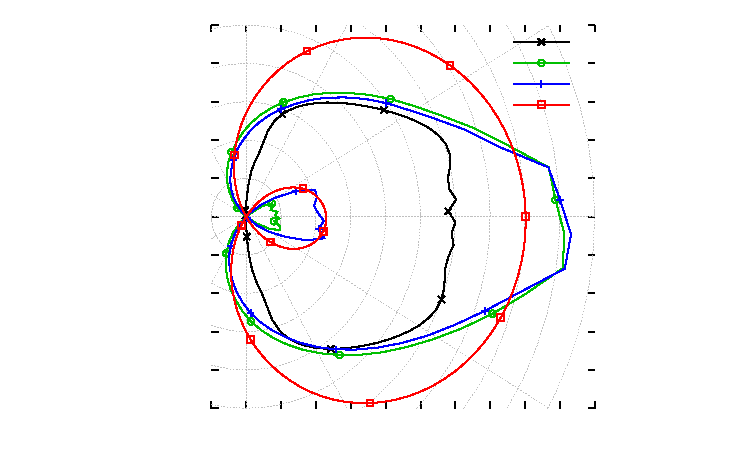
\includegraphics{/Users/seth/_thesis/figures/crashpipe2b/intens-x1-t1/intensity-x1-t1.pdf}}%
    \gplfronttext
  \end{picture}%
\endgroup

  \caption{Material temperature at $t=3$ in the 1-D blast wave problem.}
  \label{fig:1dblastMattemp}
\end{figure}

\begin{figure}[htb]
  \centering\small
  % GNUPLOT: LaTeX picture with Postscript
\begingroup
  \makeatletter
  \providecommand\color[2][]{%
    \GenericError{(gnuplot) \space\space\space\@spaces}{%
      Package color not loaded in conjunction with
      terminal option `colourtext'%
    }{See the gnuplot documentation for explanation.%
    }{Either use 'blacktext' in gnuplot or load the package
      color.sty in LaTeX.}%
    \renewcommand\color[2][]{}%
  }%
  \providecommand\includegraphics[2][]{%
    \GenericError{(gnuplot) \space\space\space\@spaces}{%
      Package graphicx or graphics not loaded%
    }{See the gnuplot documentation for explanation.%
    }{The gnuplot epslatex terminal needs graphicx.sty or graphics.sty.}%
    \renewcommand\includegraphics[2][]{}%
  }%
  \providecommand\rotatebox[2]{#2}%
  \@ifundefined{ifGPcolor}{%
    \newif\ifGPcolor
    \GPcolortrue
  }{}%
  \@ifundefined{ifGPblacktext}{%
    \newif\ifGPblacktext
    \GPblacktexttrue
  }{}%
  % define a \g@addto@macro without @ in the name:
  \let\gplgaddtomacro\g@addto@macro
  % define empty templates for all commands taking text:
  \gdef\gplbacktext{}%
  \gdef\gplfronttext{}%
  \makeatother
  \ifGPblacktext
    % no textcolor at all
    \def\colorrgb#1{}%
    \def\colorgray#1{}%
  \else
    % gray or color?
    \ifGPcolor
      \def\colorrgb#1{\color[rgb]{#1}}%
      \def\colorgray#1{\color[gray]{#1}}%
      \expandafter\def\csname LTw\endcsname{\color{white}}%
      \expandafter\def\csname LTb\endcsname{\color{black}}%
      \expandafter\def\csname LTa\endcsname{\color{black}}%
      \expandafter\def\csname LT0\endcsname{\color[rgb]{1,0,0}}%
      \expandafter\def\csname LT1\endcsname{\color[rgb]{0,1,0}}%
      \expandafter\def\csname LT2\endcsname{\color[rgb]{0,0,1}}%
      \expandafter\def\csname LT3\endcsname{\color[rgb]{1,0,1}}%
      \expandafter\def\csname LT4\endcsname{\color[rgb]{0,1,1}}%
      \expandafter\def\csname LT5\endcsname{\color[rgb]{1,1,0}}%
      \expandafter\def\csname LT6\endcsname{\color[rgb]{0,0,0}}%
      \expandafter\def\csname LT7\endcsname{\color[rgb]{1,0.3,0}}%
      \expandafter\def\csname LT8\endcsname{\color[rgb]{0.5,0.5,0.5}}%
    \else
      % gray
      \def\colorrgb#1{\color{black}}%
      \def\colorgray#1{\color[gray]{#1}}%
      \expandafter\def\csname LTw\endcsname{\color{white}}%
      \expandafter\def\csname LTb\endcsname{\color{black}}%
      \expandafter\def\csname LTa\endcsname{\color{black}}%
      \expandafter\def\csname LT0\endcsname{\color{black}}%
      \expandafter\def\csname LT1\endcsname{\color{black}}%
      \expandafter\def\csname LT2\endcsname{\color{black}}%
      \expandafter\def\csname LT3\endcsname{\color{black}}%
      \expandafter\def\csname LT4\endcsname{\color{black}}%
      \expandafter\def\csname LT5\endcsname{\color{black}}%
      \expandafter\def\csname LT6\endcsname{\color{black}}%
      \expandafter\def\csname LT7\endcsname{\color{black}}%
      \expandafter\def\csname LT8\endcsname{\color{black}}%
    \fi
  \fi
  \setlength{\unitlength}{0.0500bp}%
  \begin{picture}(7200.00,4320.00)%
    \gplgaddtomacro\gplbacktext{%
      \csname LTb\endcsname%
      \put(1910,400){\makebox(0,0)[r]{\strut{} 0.1}}%
      \put(1910,768){\makebox(0,0)[r]{\strut{} 0.08}}%
      \put(1910,1136){\makebox(0,0)[r]{\strut{} 0.06}}%
      \put(1910,1504){\makebox(0,0)[r]{\strut{} 0.04}}%
      \put(1910,1872){\makebox(0,0)[r]{\strut{} 0.02}}%
      \put(1910,2240){\makebox(0,0)[r]{\strut{} 0}}%
      \put(1910,2607){\makebox(0,0)[r]{\strut{} 0.02}}%
      \put(1910,2975){\makebox(0,0)[r]{\strut{} 0.04}}%
      \put(1910,3343){\makebox(0,0)[r]{\strut{} 0.06}}%
      \put(1910,3711){\makebox(0,0)[r]{\strut{} 0.08}}%
      \put(1910,4079){\makebox(0,0)[r]{\strut{} 0.1}}%
      \csname LTb\endcsname%
      \put(2030,200){\makebox(0,0){\strut{} 0.02}}%
      \csname LTb\endcsname%
      \put(2364,200){\makebox(0,0){\strut{} 0}}%
      \csname LTb\endcsname%
      \put(2699,200){\makebox(0,0){\strut{} 0.02}}%
      \csname LTb\endcsname%
      \put(3033,200){\makebox(0,0){\strut{} 0.04}}%
      \csname LTb\endcsname%
      \put(3368,200){\makebox(0,0){\strut{} 0.06}}%
      \csname LTb\endcsname%
      \put(3702,200){\makebox(0,0){\strut{} 0.08}}%
      \csname LTb\endcsname%
      \put(4037,200){\makebox(0,0){\strut{} 0.1}}%
      \csname LTb\endcsname%
      \put(4371,200){\makebox(0,0){\strut{} 0.12}}%
      \csname LTb\endcsname%
      \put(4706,200){\makebox(0,0){\strut{} 0.14}}%
      \csname LTb\endcsname%
      \put(5040,200){\makebox(0,0){\strut{} 0.16}}%
      \csname LTb\endcsname%
      \put(5375,200){\makebox(0,0){\strut{} 0.18}}%
      \csname LTb\endcsname%
      \put(5709,200){\makebox(0,0){\strut{} 0.2}}%
      \csname LTb\endcsname%
      \put(1330,2239){\rotatebox{-270}{\makebox(0,0){\strut{}x1 center $(1.01,3.5)$}}}%
    }%
    \gplgaddtomacro\gplfronttext{%
      \csname LTb\endcsname%
      \put(4806,3916){\makebox(0,0)[r]{\strut{}S$_{128}$}}%
      \csname LTb\endcsname%
      \put(4806,3716){\makebox(0,0)[r]{\strut{}FLAD$_{64}$}}%
      \csname LTb\endcsname%
      \put(4806,3516){\makebox(0,0)[r]{\strut{}AD$_{64}$}}%
      \csname LTb\endcsname%
      \put(4806,3316){\makebox(0,0)[r]{\strut{}FLD}}%
    }%
    \gplbacktext
    \put(0,0){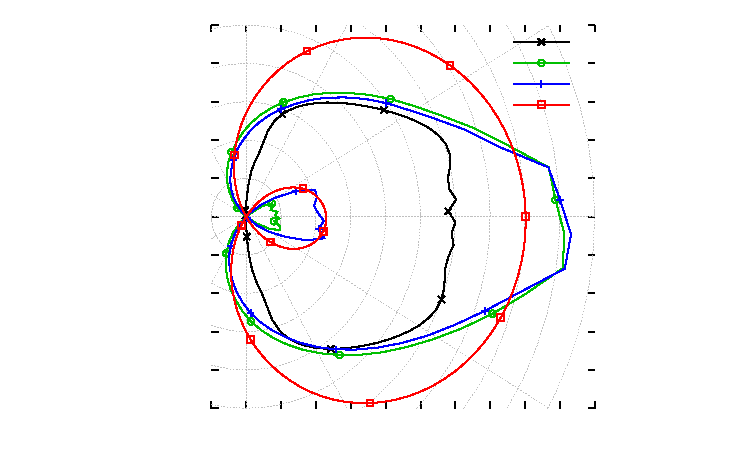
\includegraphics{/Users/seth/_thesis/figures/crashpipe2b/intens-x1-t1/intensity-x1-t1.pdf}}%
    \gplfronttext
  \end{picture}%
\endgroup

  \caption{Wavefront position of $\phi$ in 1-D blast wave problem.}
  \label{fig:1dblastWavefront}
\end{figure}

%%%%%%%%%%%%%%%%%%%%%%%%%%%%%%%%%%%%%%%%%%%%%%%%%%%%%%%%%%%%%%%%%%%%%%%%%%%%%%%%
\section{Flatland pipe with internal source}

\begin{figure}[htb]
  \centering\small
  \subfloat[Centerline view]{%
    \hspace{-.25in}%
    % GNUPLOT: LaTeX picture with Postscript
\begingroup
  \makeatletter
  \providecommand\color[2][]{%
    \GenericError{(gnuplot) \space\space\space\@spaces}{%
      Package color not loaded in conjunction with
      terminal option `colourtext'%
    }{See the gnuplot documentation for explanation.%
    }{Either use 'blacktext' in gnuplot or load the package
      color.sty in LaTeX.}%
    \renewcommand\color[2][]{}%
  }%
  \providecommand\includegraphics[2][]{%
    \GenericError{(gnuplot) \space\space\space\@spaces}{%
      Package graphicx or graphics not loaded%
    }{See the gnuplot documentation for explanation.%
    }{The gnuplot epslatex terminal needs graphicx.sty or graphics.sty.}%
    \renewcommand\includegraphics[2][]{}%
  }%
  \providecommand\rotatebox[2]{#2}%
  \@ifundefined{ifGPcolor}{%
    \newif\ifGPcolor
    \GPcolortrue
  }{}%
  \@ifundefined{ifGPblacktext}{%
    \newif\ifGPblacktext
    \GPblacktexttrue
  }{}%
  % define a \g@addto@macro without @ in the name:
  \let\gplgaddtomacro\g@addto@macro
  % define empty templates for all commands taking text:
  \gdef\gplbacktext{}%
  \gdef\gplfronttext{}%
  \makeatother
  \ifGPblacktext
    % no textcolor at all
    \def\colorrgb#1{}%
    \def\colorgray#1{}%
  \else
    % gray or color?
    \ifGPcolor
      \def\colorrgb#1{\color[rgb]{#1}}%
      \def\colorgray#1{\color[gray]{#1}}%
      \expandafter\def\csname LTw\endcsname{\color{white}}%
      \expandafter\def\csname LTb\endcsname{\color{black}}%
      \expandafter\def\csname LTa\endcsname{\color{black}}%
      \expandafter\def\csname LT0\endcsname{\color[rgb]{1,0,0}}%
      \expandafter\def\csname LT1\endcsname{\color[rgb]{0,1,0}}%
      \expandafter\def\csname LT2\endcsname{\color[rgb]{0,0,1}}%
      \expandafter\def\csname LT3\endcsname{\color[rgb]{1,0,1}}%
      \expandafter\def\csname LT4\endcsname{\color[rgb]{0,1,1}}%
      \expandafter\def\csname LT5\endcsname{\color[rgb]{1,1,0}}%
      \expandafter\def\csname LT6\endcsname{\color[rgb]{0,0,0}}%
      \expandafter\def\csname LT7\endcsname{\color[rgb]{1,0.3,0}}%
      \expandafter\def\csname LT8\endcsname{\color[rgb]{0.5,0.5,0.5}}%
    \else
      % gray
      \def\colorrgb#1{\color{black}}%
      \def\colorgray#1{\color[gray]{#1}}%
      \expandafter\def\csname LTw\endcsname{\color{white}}%
      \expandafter\def\csname LTb\endcsname{\color{black}}%
      \expandafter\def\csname LTa\endcsname{\color{black}}%
      \expandafter\def\csname LT0\endcsname{\color{black}}%
      \expandafter\def\csname LT1\endcsname{\color{black}}%
      \expandafter\def\csname LT2\endcsname{\color{black}}%
      \expandafter\def\csname LT3\endcsname{\color{black}}%
      \expandafter\def\csname LT4\endcsname{\color{black}}%
      \expandafter\def\csname LT5\endcsname{\color{black}}%
      \expandafter\def\csname LT6\endcsname{\color{black}}%
      \expandafter\def\csname LT7\endcsname{\color{black}}%
      \expandafter\def\csname LT8\endcsname{\color{black}}%
    \fi
  \fi
  \setlength{\unitlength}{0.0500bp}%
  \begin{picture}(7200.00,4320.00)%
    \gplgaddtomacro\gplbacktext{%
      \csname LTb\endcsname%
      \put(1910,400){\makebox(0,0)[r]{\strut{} 0.1}}%
      \put(1910,768){\makebox(0,0)[r]{\strut{} 0.08}}%
      \put(1910,1136){\makebox(0,0)[r]{\strut{} 0.06}}%
      \put(1910,1504){\makebox(0,0)[r]{\strut{} 0.04}}%
      \put(1910,1872){\makebox(0,0)[r]{\strut{} 0.02}}%
      \put(1910,2240){\makebox(0,0)[r]{\strut{} 0}}%
      \put(1910,2607){\makebox(0,0)[r]{\strut{} 0.02}}%
      \put(1910,2975){\makebox(0,0)[r]{\strut{} 0.04}}%
      \put(1910,3343){\makebox(0,0)[r]{\strut{} 0.06}}%
      \put(1910,3711){\makebox(0,0)[r]{\strut{} 0.08}}%
      \put(1910,4079){\makebox(0,0)[r]{\strut{} 0.1}}%
      \csname LTb\endcsname%
      \put(2030,200){\makebox(0,0){\strut{} 0.02}}%
      \csname LTb\endcsname%
      \put(2364,200){\makebox(0,0){\strut{} 0}}%
      \csname LTb\endcsname%
      \put(2699,200){\makebox(0,0){\strut{} 0.02}}%
      \csname LTb\endcsname%
      \put(3033,200){\makebox(0,0){\strut{} 0.04}}%
      \csname LTb\endcsname%
      \put(3368,200){\makebox(0,0){\strut{} 0.06}}%
      \csname LTb\endcsname%
      \put(3702,200){\makebox(0,0){\strut{} 0.08}}%
      \csname LTb\endcsname%
      \put(4037,200){\makebox(0,0){\strut{} 0.1}}%
      \csname LTb\endcsname%
      \put(4371,200){\makebox(0,0){\strut{} 0.12}}%
      \csname LTb\endcsname%
      \put(4706,200){\makebox(0,0){\strut{} 0.14}}%
      \csname LTb\endcsname%
      \put(5040,200){\makebox(0,0){\strut{} 0.16}}%
      \csname LTb\endcsname%
      \put(5375,200){\makebox(0,0){\strut{} 0.18}}%
      \csname LTb\endcsname%
      \put(5709,200){\makebox(0,0){\strut{} 0.2}}%
      \csname LTb\endcsname%
      \put(1330,2239){\rotatebox{-270}{\makebox(0,0){\strut{}x1 center $(1.01,3.5)$}}}%
    }%
    \gplgaddtomacro\gplfronttext{%
      \csname LTb\endcsname%
      \put(4806,3916){\makebox(0,0)[r]{\strut{}S$_{128}$}}%
      \csname LTb\endcsname%
      \put(4806,3716){\makebox(0,0)[r]{\strut{}FLAD$_{64}$}}%
      \csname LTb\endcsname%
      \put(4806,3516){\makebox(0,0)[r]{\strut{}AD$_{64}$}}%
      \csname LTb\endcsname%
      \put(4806,3316){\makebox(0,0)[r]{\strut{}FLD}}%
    }%
    \gplbacktext
    \put(0,0){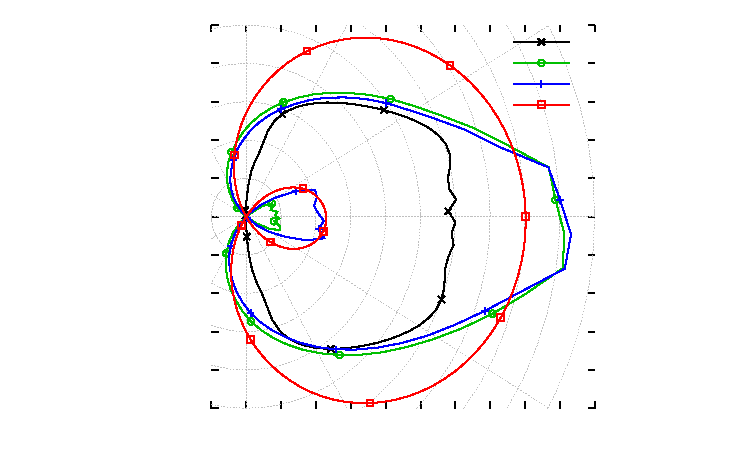
\includegraphics{/Users/seth/_thesis/figures/crashpipe2b/intens-x1-t1/intensity-x1-t1.pdf}}%
    \gplfronttext
  \end{picture}%
\endgroup

  }%
  \subfloat[Orthogonal view]{%
    \hspace{-.25in}%
    % GNUPLOT: LaTeX picture with Postscript
\begingroup
  \makeatletter
  \providecommand\color[2][]{%
    \GenericError{(gnuplot) \space\space\space\@spaces}{%
      Package color not loaded in conjunction with
      terminal option `colourtext'%
    }{See the gnuplot documentation for explanation.%
    }{Either use 'blacktext' in gnuplot or load the package
      color.sty in LaTeX.}%
    \renewcommand\color[2][]{}%
  }%
  \providecommand\includegraphics[2][]{%
    \GenericError{(gnuplot) \space\space\space\@spaces}{%
      Package graphicx or graphics not loaded%
    }{See the gnuplot documentation for explanation.%
    }{The gnuplot epslatex terminal needs graphicx.sty or graphics.sty.}%
    \renewcommand\includegraphics[2][]{}%
  }%
  \providecommand\rotatebox[2]{#2}%
  \@ifundefined{ifGPcolor}{%
    \newif\ifGPcolor
    \GPcolortrue
  }{}%
  \@ifundefined{ifGPblacktext}{%
    \newif\ifGPblacktext
    \GPblacktexttrue
  }{}%
  % define a \g@addto@macro without @ in the name:
  \let\gplgaddtomacro\g@addto@macro
  % define empty templates for all commands taking text:
  \gdef\gplbacktext{}%
  \gdef\gplfronttext{}%
  \makeatother
  \ifGPblacktext
    % no textcolor at all
    \def\colorrgb#1{}%
    \def\colorgray#1{}%
  \else
    % gray or color?
    \ifGPcolor
      \def\colorrgb#1{\color[rgb]{#1}}%
      \def\colorgray#1{\color[gray]{#1}}%
      \expandafter\def\csname LTw\endcsname{\color{white}}%
      \expandafter\def\csname LTb\endcsname{\color{black}}%
      \expandafter\def\csname LTa\endcsname{\color{black}}%
      \expandafter\def\csname LT0\endcsname{\color[rgb]{1,0,0}}%
      \expandafter\def\csname LT1\endcsname{\color[rgb]{0,1,0}}%
      \expandafter\def\csname LT2\endcsname{\color[rgb]{0,0,1}}%
      \expandafter\def\csname LT3\endcsname{\color[rgb]{1,0,1}}%
      \expandafter\def\csname LT4\endcsname{\color[rgb]{0,1,1}}%
      \expandafter\def\csname LT5\endcsname{\color[rgb]{1,1,0}}%
      \expandafter\def\csname LT6\endcsname{\color[rgb]{0,0,0}}%
      \expandafter\def\csname LT7\endcsname{\color[rgb]{1,0.3,0}}%
      \expandafter\def\csname LT8\endcsname{\color[rgb]{0.5,0.5,0.5}}%
    \else
      % gray
      \def\colorrgb#1{\color{black}}%
      \def\colorgray#1{\color[gray]{#1}}%
      \expandafter\def\csname LTw\endcsname{\color{white}}%
      \expandafter\def\csname LTb\endcsname{\color{black}}%
      \expandafter\def\csname LTa\endcsname{\color{black}}%
      \expandafter\def\csname LT0\endcsname{\color{black}}%
      \expandafter\def\csname LT1\endcsname{\color{black}}%
      \expandafter\def\csname LT2\endcsname{\color{black}}%
      \expandafter\def\csname LT3\endcsname{\color{black}}%
      \expandafter\def\csname LT4\endcsname{\color{black}}%
      \expandafter\def\csname LT5\endcsname{\color{black}}%
      \expandafter\def\csname LT6\endcsname{\color{black}}%
      \expandafter\def\csname LT7\endcsname{\color{black}}%
      \expandafter\def\csname LT8\endcsname{\color{black}}%
    \fi
  \fi
  \setlength{\unitlength}{0.0500bp}%
  \begin{picture}(7200.00,4320.00)%
    \gplgaddtomacro\gplbacktext{%
      \csname LTb\endcsname%
      \put(1910,400){\makebox(0,0)[r]{\strut{} 0.1}}%
      \put(1910,768){\makebox(0,0)[r]{\strut{} 0.08}}%
      \put(1910,1136){\makebox(0,0)[r]{\strut{} 0.06}}%
      \put(1910,1504){\makebox(0,0)[r]{\strut{} 0.04}}%
      \put(1910,1872){\makebox(0,0)[r]{\strut{} 0.02}}%
      \put(1910,2240){\makebox(0,0)[r]{\strut{} 0}}%
      \put(1910,2607){\makebox(0,0)[r]{\strut{} 0.02}}%
      \put(1910,2975){\makebox(0,0)[r]{\strut{} 0.04}}%
      \put(1910,3343){\makebox(0,0)[r]{\strut{} 0.06}}%
      \put(1910,3711){\makebox(0,0)[r]{\strut{} 0.08}}%
      \put(1910,4079){\makebox(0,0)[r]{\strut{} 0.1}}%
      \csname LTb\endcsname%
      \put(2030,200){\makebox(0,0){\strut{} 0.02}}%
      \csname LTb\endcsname%
      \put(2364,200){\makebox(0,0){\strut{} 0}}%
      \csname LTb\endcsname%
      \put(2699,200){\makebox(0,0){\strut{} 0.02}}%
      \csname LTb\endcsname%
      \put(3033,200){\makebox(0,0){\strut{} 0.04}}%
      \csname LTb\endcsname%
      \put(3368,200){\makebox(0,0){\strut{} 0.06}}%
      \csname LTb\endcsname%
      \put(3702,200){\makebox(0,0){\strut{} 0.08}}%
      \csname LTb\endcsname%
      \put(4037,200){\makebox(0,0){\strut{} 0.1}}%
      \csname LTb\endcsname%
      \put(4371,200){\makebox(0,0){\strut{} 0.12}}%
      \csname LTb\endcsname%
      \put(4706,200){\makebox(0,0){\strut{} 0.14}}%
      \csname LTb\endcsname%
      \put(5040,200){\makebox(0,0){\strut{} 0.16}}%
      \csname LTb\endcsname%
      \put(5375,200){\makebox(0,0){\strut{} 0.18}}%
      \csname LTb\endcsname%
      \put(5709,200){\makebox(0,0){\strut{} 0.2}}%
      \csname LTb\endcsname%
      \put(1330,2239){\rotatebox{-270}{\makebox(0,0){\strut{}x1 center $(1.01,3.5)$}}}%
    }%
    \gplgaddtomacro\gplfronttext{%
      \csname LTb\endcsname%
      \put(4806,3916){\makebox(0,0)[r]{\strut{}S$_{128}$}}%
      \csname LTb\endcsname%
      \put(4806,3716){\makebox(0,0)[r]{\strut{}FLAD$_{64}$}}%
      \csname LTb\endcsname%
      \put(4806,3516){\makebox(0,0)[r]{\strut{}AD$_{64}$}}%
      \csname LTb\endcsname%
      \put(4806,3316){\makebox(0,0)[r]{\strut{}FLD}}%
    }%
    \gplbacktext
    \put(0,0){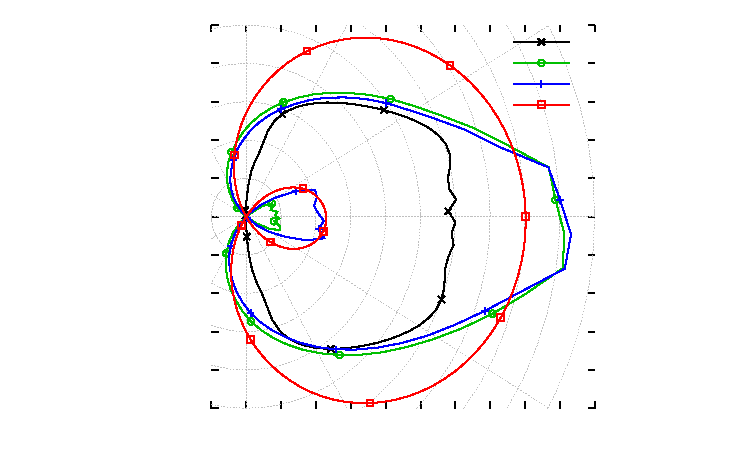
\includegraphics{/Users/seth/_thesis/figures/crashpipe2b/intens-x1-t1/intensity-x1-t1.pdf}}%
    \gplfronttext
  \end{picture}%
\endgroup

  }%
  \caption{Material temperature at $t=3$ in the flatland source problem.}
  \label{fig:crashaltMattemp}
\end{figure}

\begin{figure}[htb]
  \centering\small
  % GNUPLOT: LaTeX picture with Postscript
\begingroup
  \makeatletter
  \providecommand\color[2][]{%
    \GenericError{(gnuplot) \space\space\space\@spaces}{%
      Package color not loaded in conjunction with
      terminal option `colourtext'%
    }{See the gnuplot documentation for explanation.%
    }{Either use 'blacktext' in gnuplot or load the package
      color.sty in LaTeX.}%
    \renewcommand\color[2][]{}%
  }%
  \providecommand\includegraphics[2][]{%
    \GenericError{(gnuplot) \space\space\space\@spaces}{%
      Package graphicx or graphics not loaded%
    }{See the gnuplot documentation for explanation.%
    }{The gnuplot epslatex terminal needs graphicx.sty or graphics.sty.}%
    \renewcommand\includegraphics[2][]{}%
  }%
  \providecommand\rotatebox[2]{#2}%
  \@ifundefined{ifGPcolor}{%
    \newif\ifGPcolor
    \GPcolortrue
  }{}%
  \@ifundefined{ifGPblacktext}{%
    \newif\ifGPblacktext
    \GPblacktexttrue
  }{}%
  % define a \g@addto@macro without @ in the name:
  \let\gplgaddtomacro\g@addto@macro
  % define empty templates for all commands taking text:
  \gdef\gplbacktext{}%
  \gdef\gplfronttext{}%
  \makeatother
  \ifGPblacktext
    % no textcolor at all
    \def\colorrgb#1{}%
    \def\colorgray#1{}%
  \else
    % gray or color?
    \ifGPcolor
      \def\colorrgb#1{\color[rgb]{#1}}%
      \def\colorgray#1{\color[gray]{#1}}%
      \expandafter\def\csname LTw\endcsname{\color{white}}%
      \expandafter\def\csname LTb\endcsname{\color{black}}%
      \expandafter\def\csname LTa\endcsname{\color{black}}%
      \expandafter\def\csname LT0\endcsname{\color[rgb]{1,0,0}}%
      \expandafter\def\csname LT1\endcsname{\color[rgb]{0,1,0}}%
      \expandafter\def\csname LT2\endcsname{\color[rgb]{0,0,1}}%
      \expandafter\def\csname LT3\endcsname{\color[rgb]{1,0,1}}%
      \expandafter\def\csname LT4\endcsname{\color[rgb]{0,1,1}}%
      \expandafter\def\csname LT5\endcsname{\color[rgb]{1,1,0}}%
      \expandafter\def\csname LT6\endcsname{\color[rgb]{0,0,0}}%
      \expandafter\def\csname LT7\endcsname{\color[rgb]{1,0.3,0}}%
      \expandafter\def\csname LT8\endcsname{\color[rgb]{0.5,0.5,0.5}}%
    \else
      % gray
      \def\colorrgb#1{\color{black}}%
      \def\colorgray#1{\color[gray]{#1}}%
      \expandafter\def\csname LTw\endcsname{\color{white}}%
      \expandafter\def\csname LTb\endcsname{\color{black}}%
      \expandafter\def\csname LTa\endcsname{\color{black}}%
      \expandafter\def\csname LT0\endcsname{\color{black}}%
      \expandafter\def\csname LT1\endcsname{\color{black}}%
      \expandafter\def\csname LT2\endcsname{\color{black}}%
      \expandafter\def\csname LT3\endcsname{\color{black}}%
      \expandafter\def\csname LT4\endcsname{\color{black}}%
      \expandafter\def\csname LT5\endcsname{\color{black}}%
      \expandafter\def\csname LT6\endcsname{\color{black}}%
      \expandafter\def\csname LT7\endcsname{\color{black}}%
      \expandafter\def\csname LT8\endcsname{\color{black}}%
    \fi
  \fi
  \setlength{\unitlength}{0.0500bp}%
  \begin{picture}(7200.00,4320.00)%
    \gplgaddtomacro\gplbacktext{%
      \csname LTb\endcsname%
      \put(1910,400){\makebox(0,0)[r]{\strut{} 0.1}}%
      \put(1910,768){\makebox(0,0)[r]{\strut{} 0.08}}%
      \put(1910,1136){\makebox(0,0)[r]{\strut{} 0.06}}%
      \put(1910,1504){\makebox(0,0)[r]{\strut{} 0.04}}%
      \put(1910,1872){\makebox(0,0)[r]{\strut{} 0.02}}%
      \put(1910,2240){\makebox(0,0)[r]{\strut{} 0}}%
      \put(1910,2607){\makebox(0,0)[r]{\strut{} 0.02}}%
      \put(1910,2975){\makebox(0,0)[r]{\strut{} 0.04}}%
      \put(1910,3343){\makebox(0,0)[r]{\strut{} 0.06}}%
      \put(1910,3711){\makebox(0,0)[r]{\strut{} 0.08}}%
      \put(1910,4079){\makebox(0,0)[r]{\strut{} 0.1}}%
      \csname LTb\endcsname%
      \put(2030,200){\makebox(0,0){\strut{} 0.02}}%
      \csname LTb\endcsname%
      \put(2364,200){\makebox(0,0){\strut{} 0}}%
      \csname LTb\endcsname%
      \put(2699,200){\makebox(0,0){\strut{} 0.02}}%
      \csname LTb\endcsname%
      \put(3033,200){\makebox(0,0){\strut{} 0.04}}%
      \csname LTb\endcsname%
      \put(3368,200){\makebox(0,0){\strut{} 0.06}}%
      \csname LTb\endcsname%
      \put(3702,200){\makebox(0,0){\strut{} 0.08}}%
      \csname LTb\endcsname%
      \put(4037,200){\makebox(0,0){\strut{} 0.1}}%
      \csname LTb\endcsname%
      \put(4371,200){\makebox(0,0){\strut{} 0.12}}%
      \csname LTb\endcsname%
      \put(4706,200){\makebox(0,0){\strut{} 0.14}}%
      \csname LTb\endcsname%
      \put(5040,200){\makebox(0,0){\strut{} 0.16}}%
      \csname LTb\endcsname%
      \put(5375,200){\makebox(0,0){\strut{} 0.18}}%
      \csname LTb\endcsname%
      \put(5709,200){\makebox(0,0){\strut{} 0.2}}%
      \csname LTb\endcsname%
      \put(1330,2239){\rotatebox{-270}{\makebox(0,0){\strut{}x1 center $(1.01,3.5)$}}}%
    }%
    \gplgaddtomacro\gplfronttext{%
      \csname LTb\endcsname%
      \put(4806,3916){\makebox(0,0)[r]{\strut{}S$_{128}$}}%
      \csname LTb\endcsname%
      \put(4806,3716){\makebox(0,0)[r]{\strut{}FLAD$_{64}$}}%
      \csname LTb\endcsname%
      \put(4806,3516){\makebox(0,0)[r]{\strut{}AD$_{64}$}}%
      \csname LTb\endcsname%
      \put(4806,3316){\makebox(0,0)[r]{\strut{}FLD}}%
    }%
    \gplbacktext
    \put(0,0){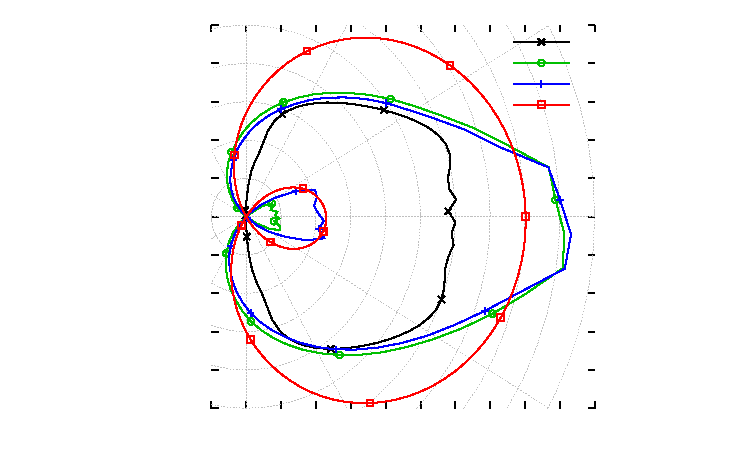
\includegraphics{/Users/seth/_thesis/figures/crashpipe2b/intens-x1-t1/intensity-x1-t1.pdf}}%
    \gplfronttext
  \end{picture}%
\endgroup

  \caption{Wavefront position of $\phi$ in the flatland source problem.}
  \label{fig:crashaltWavefront}
\end{figure}


\begin{figure}[htb]
  \centering\small
  \subfloat[Centerline view]{%
    \hspace{-.25in}%
    % GNUPLOT: LaTeX picture with Postscript
\begingroup
  \makeatletter
  \providecommand\color[2][]{%
    \GenericError{(gnuplot) \space\space\space\@spaces}{%
      Package color not loaded in conjunction with
      terminal option `colourtext'%
    }{See the gnuplot documentation for explanation.%
    }{Either use 'blacktext' in gnuplot or load the package
      color.sty in LaTeX.}%
    \renewcommand\color[2][]{}%
  }%
  \providecommand\includegraphics[2][]{%
    \GenericError{(gnuplot) \space\space\space\@spaces}{%
      Package graphicx or graphics not loaded%
    }{See the gnuplot documentation for explanation.%
    }{The gnuplot epslatex terminal needs graphicx.sty or graphics.sty.}%
    \renewcommand\includegraphics[2][]{}%
  }%
  \providecommand\rotatebox[2]{#2}%
  \@ifundefined{ifGPcolor}{%
    \newif\ifGPcolor
    \GPcolortrue
  }{}%
  \@ifundefined{ifGPblacktext}{%
    \newif\ifGPblacktext
    \GPblacktexttrue
  }{}%
  % define a \g@addto@macro without @ in the name:
  \let\gplgaddtomacro\g@addto@macro
  % define empty templates for all commands taking text:
  \gdef\gplbacktext{}%
  \gdef\gplfronttext{}%
  \makeatother
  \ifGPblacktext
    % no textcolor at all
    \def\colorrgb#1{}%
    \def\colorgray#1{}%
  \else
    % gray or color?
    \ifGPcolor
      \def\colorrgb#1{\color[rgb]{#1}}%
      \def\colorgray#1{\color[gray]{#1}}%
      \expandafter\def\csname LTw\endcsname{\color{white}}%
      \expandafter\def\csname LTb\endcsname{\color{black}}%
      \expandafter\def\csname LTa\endcsname{\color{black}}%
      \expandafter\def\csname LT0\endcsname{\color[rgb]{1,0,0}}%
      \expandafter\def\csname LT1\endcsname{\color[rgb]{0,1,0}}%
      \expandafter\def\csname LT2\endcsname{\color[rgb]{0,0,1}}%
      \expandafter\def\csname LT3\endcsname{\color[rgb]{1,0,1}}%
      \expandafter\def\csname LT4\endcsname{\color[rgb]{0,1,1}}%
      \expandafter\def\csname LT5\endcsname{\color[rgb]{1,1,0}}%
      \expandafter\def\csname LT6\endcsname{\color[rgb]{0,0,0}}%
      \expandafter\def\csname LT7\endcsname{\color[rgb]{1,0.3,0}}%
      \expandafter\def\csname LT8\endcsname{\color[rgb]{0.5,0.5,0.5}}%
    \else
      % gray
      \def\colorrgb#1{\color{black}}%
      \def\colorgray#1{\color[gray]{#1}}%
      \expandafter\def\csname LTw\endcsname{\color{white}}%
      \expandafter\def\csname LTb\endcsname{\color{black}}%
      \expandafter\def\csname LTa\endcsname{\color{black}}%
      \expandafter\def\csname LT0\endcsname{\color{black}}%
      \expandafter\def\csname LT1\endcsname{\color{black}}%
      \expandafter\def\csname LT2\endcsname{\color{black}}%
      \expandafter\def\csname LT3\endcsname{\color{black}}%
      \expandafter\def\csname LT4\endcsname{\color{black}}%
      \expandafter\def\csname LT5\endcsname{\color{black}}%
      \expandafter\def\csname LT6\endcsname{\color{black}}%
      \expandafter\def\csname LT7\endcsname{\color{black}}%
      \expandafter\def\csname LT8\endcsname{\color{black}}%
    \fi
  \fi
  \setlength{\unitlength}{0.0500bp}%
  \begin{picture}(7200.00,4320.00)%
    \gplgaddtomacro\gplbacktext{%
      \csname LTb\endcsname%
      \put(1910,400){\makebox(0,0)[r]{\strut{} 0.1}}%
      \put(1910,768){\makebox(0,0)[r]{\strut{} 0.08}}%
      \put(1910,1136){\makebox(0,0)[r]{\strut{} 0.06}}%
      \put(1910,1504){\makebox(0,0)[r]{\strut{} 0.04}}%
      \put(1910,1872){\makebox(0,0)[r]{\strut{} 0.02}}%
      \put(1910,2240){\makebox(0,0)[r]{\strut{} 0}}%
      \put(1910,2607){\makebox(0,0)[r]{\strut{} 0.02}}%
      \put(1910,2975){\makebox(0,0)[r]{\strut{} 0.04}}%
      \put(1910,3343){\makebox(0,0)[r]{\strut{} 0.06}}%
      \put(1910,3711){\makebox(0,0)[r]{\strut{} 0.08}}%
      \put(1910,4079){\makebox(0,0)[r]{\strut{} 0.1}}%
      \csname LTb\endcsname%
      \put(2030,200){\makebox(0,0){\strut{} 0.02}}%
      \csname LTb\endcsname%
      \put(2364,200){\makebox(0,0){\strut{} 0}}%
      \csname LTb\endcsname%
      \put(2699,200){\makebox(0,0){\strut{} 0.02}}%
      \csname LTb\endcsname%
      \put(3033,200){\makebox(0,0){\strut{} 0.04}}%
      \csname LTb\endcsname%
      \put(3368,200){\makebox(0,0){\strut{} 0.06}}%
      \csname LTb\endcsname%
      \put(3702,200){\makebox(0,0){\strut{} 0.08}}%
      \csname LTb\endcsname%
      \put(4037,200){\makebox(0,0){\strut{} 0.1}}%
      \csname LTb\endcsname%
      \put(4371,200){\makebox(0,0){\strut{} 0.12}}%
      \csname LTb\endcsname%
      \put(4706,200){\makebox(0,0){\strut{} 0.14}}%
      \csname LTb\endcsname%
      \put(5040,200){\makebox(0,0){\strut{} 0.16}}%
      \csname LTb\endcsname%
      \put(5375,200){\makebox(0,0){\strut{} 0.18}}%
      \csname LTb\endcsname%
      \put(5709,200){\makebox(0,0){\strut{} 0.2}}%
      \csname LTb\endcsname%
      \put(1330,2239){\rotatebox{-270}{\makebox(0,0){\strut{}x1 center $(1.01,3.5)$}}}%
    }%
    \gplgaddtomacro\gplfronttext{%
      \csname LTb\endcsname%
      \put(4806,3916){\makebox(0,0)[r]{\strut{}S$_{128}$}}%
      \csname LTb\endcsname%
      \put(4806,3716){\makebox(0,0)[r]{\strut{}FLAD$_{64}$}}%
      \csname LTb\endcsname%
      \put(4806,3516){\makebox(0,0)[r]{\strut{}AD$_{64}$}}%
      \csname LTb\endcsname%
      \put(4806,3316){\makebox(0,0)[r]{\strut{}FLD}}%
    }%
    \gplbacktext
    \put(0,0){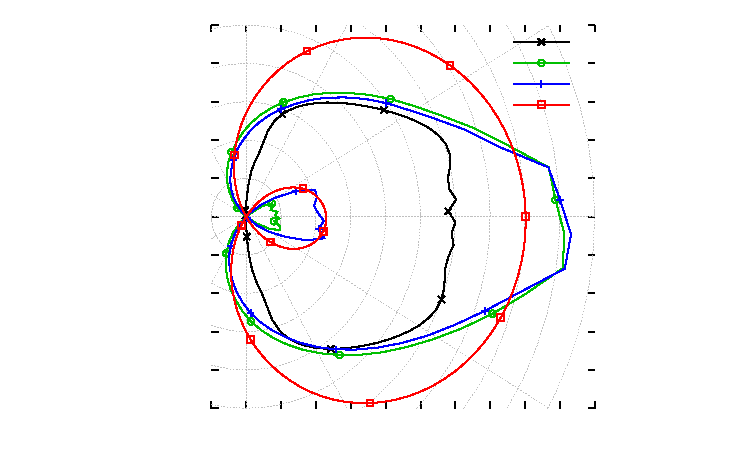
\includegraphics{/Users/seth/_thesis/figures/crashpipe2b/intens-x1-t1/intensity-x1-t1.pdf}}%
    \gplfronttext
  \end{picture}%
\endgroup

  }%
  \subfloat[Orthogonal view]{%
    \hspace{-.25in}%
    % GNUPLOT: LaTeX picture with Postscript
\begingroup
  \makeatletter
  \providecommand\color[2][]{%
    \GenericError{(gnuplot) \space\space\space\@spaces}{%
      Package color not loaded in conjunction with
      terminal option `colourtext'%
    }{See the gnuplot documentation for explanation.%
    }{Either use 'blacktext' in gnuplot or load the package
      color.sty in LaTeX.}%
    \renewcommand\color[2][]{}%
  }%
  \providecommand\includegraphics[2][]{%
    \GenericError{(gnuplot) \space\space\space\@spaces}{%
      Package graphicx or graphics not loaded%
    }{See the gnuplot documentation for explanation.%
    }{The gnuplot epslatex terminal needs graphicx.sty or graphics.sty.}%
    \renewcommand\includegraphics[2][]{}%
  }%
  \providecommand\rotatebox[2]{#2}%
  \@ifundefined{ifGPcolor}{%
    \newif\ifGPcolor
    \GPcolortrue
  }{}%
  \@ifundefined{ifGPblacktext}{%
    \newif\ifGPblacktext
    \GPblacktexttrue
  }{}%
  % define a \g@addto@macro without @ in the name:
  \let\gplgaddtomacro\g@addto@macro
  % define empty templates for all commands taking text:
  \gdef\gplbacktext{}%
  \gdef\gplfronttext{}%
  \makeatother
  \ifGPblacktext
    % no textcolor at all
    \def\colorrgb#1{}%
    \def\colorgray#1{}%
  \else
    % gray or color?
    \ifGPcolor
      \def\colorrgb#1{\color[rgb]{#1}}%
      \def\colorgray#1{\color[gray]{#1}}%
      \expandafter\def\csname LTw\endcsname{\color{white}}%
      \expandafter\def\csname LTb\endcsname{\color{black}}%
      \expandafter\def\csname LTa\endcsname{\color{black}}%
      \expandafter\def\csname LT0\endcsname{\color[rgb]{1,0,0}}%
      \expandafter\def\csname LT1\endcsname{\color[rgb]{0,1,0}}%
      \expandafter\def\csname LT2\endcsname{\color[rgb]{0,0,1}}%
      \expandafter\def\csname LT3\endcsname{\color[rgb]{1,0,1}}%
      \expandafter\def\csname LT4\endcsname{\color[rgb]{0,1,1}}%
      \expandafter\def\csname LT5\endcsname{\color[rgb]{1,1,0}}%
      \expandafter\def\csname LT6\endcsname{\color[rgb]{0,0,0}}%
      \expandafter\def\csname LT7\endcsname{\color[rgb]{1,0.3,0}}%
      \expandafter\def\csname LT8\endcsname{\color[rgb]{0.5,0.5,0.5}}%
    \else
      % gray
      \def\colorrgb#1{\color{black}}%
      \def\colorgray#1{\color[gray]{#1}}%
      \expandafter\def\csname LTw\endcsname{\color{white}}%
      \expandafter\def\csname LTb\endcsname{\color{black}}%
      \expandafter\def\csname LTa\endcsname{\color{black}}%
      \expandafter\def\csname LT0\endcsname{\color{black}}%
      \expandafter\def\csname LT1\endcsname{\color{black}}%
      \expandafter\def\csname LT2\endcsname{\color{black}}%
      \expandafter\def\csname LT3\endcsname{\color{black}}%
      \expandafter\def\csname LT4\endcsname{\color{black}}%
      \expandafter\def\csname LT5\endcsname{\color{black}}%
      \expandafter\def\csname LT6\endcsname{\color{black}}%
      \expandafter\def\csname LT7\endcsname{\color{black}}%
      \expandafter\def\csname LT8\endcsname{\color{black}}%
    \fi
  \fi
  \setlength{\unitlength}{0.0500bp}%
  \begin{picture}(7200.00,4320.00)%
    \gplgaddtomacro\gplbacktext{%
      \csname LTb\endcsname%
      \put(1910,400){\makebox(0,0)[r]{\strut{} 0.1}}%
      \put(1910,768){\makebox(0,0)[r]{\strut{} 0.08}}%
      \put(1910,1136){\makebox(0,0)[r]{\strut{} 0.06}}%
      \put(1910,1504){\makebox(0,0)[r]{\strut{} 0.04}}%
      \put(1910,1872){\makebox(0,0)[r]{\strut{} 0.02}}%
      \put(1910,2240){\makebox(0,0)[r]{\strut{} 0}}%
      \put(1910,2607){\makebox(0,0)[r]{\strut{} 0.02}}%
      \put(1910,2975){\makebox(0,0)[r]{\strut{} 0.04}}%
      \put(1910,3343){\makebox(0,0)[r]{\strut{} 0.06}}%
      \put(1910,3711){\makebox(0,0)[r]{\strut{} 0.08}}%
      \put(1910,4079){\makebox(0,0)[r]{\strut{} 0.1}}%
      \csname LTb\endcsname%
      \put(2030,200){\makebox(0,0){\strut{} 0.02}}%
      \csname LTb\endcsname%
      \put(2364,200){\makebox(0,0){\strut{} 0}}%
      \csname LTb\endcsname%
      \put(2699,200){\makebox(0,0){\strut{} 0.02}}%
      \csname LTb\endcsname%
      \put(3033,200){\makebox(0,0){\strut{} 0.04}}%
      \csname LTb\endcsname%
      \put(3368,200){\makebox(0,0){\strut{} 0.06}}%
      \csname LTb\endcsname%
      \put(3702,200){\makebox(0,0){\strut{} 0.08}}%
      \csname LTb\endcsname%
      \put(4037,200){\makebox(0,0){\strut{} 0.1}}%
      \csname LTb\endcsname%
      \put(4371,200){\makebox(0,0){\strut{} 0.12}}%
      \csname LTb\endcsname%
      \put(4706,200){\makebox(0,0){\strut{} 0.14}}%
      \csname LTb\endcsname%
      \put(5040,200){\makebox(0,0){\strut{} 0.16}}%
      \csname LTb\endcsname%
      \put(5375,200){\makebox(0,0){\strut{} 0.18}}%
      \csname LTb\endcsname%
      \put(5709,200){\makebox(0,0){\strut{} 0.2}}%
      \csname LTb\endcsname%
      \put(1330,2239){\rotatebox{-270}{\makebox(0,0){\strut{}x1 center $(1.01,3.5)$}}}%
    }%
    \gplgaddtomacro\gplfronttext{%
      \csname LTb\endcsname%
      \put(4806,3916){\makebox(0,0)[r]{\strut{}S$_{128}$}}%
      \csname LTb\endcsname%
      \put(4806,3716){\makebox(0,0)[r]{\strut{}FLAD$_{64}$}}%
      \csname LTb\endcsname%
      \put(4806,3516){\makebox(0,0)[r]{\strut{}AD$_{64}$}}%
      \csname LTb\endcsname%
      \put(4806,3316){\makebox(0,0)[r]{\strut{}FLD}}%
    }%
    \gplbacktext
    \put(0,0){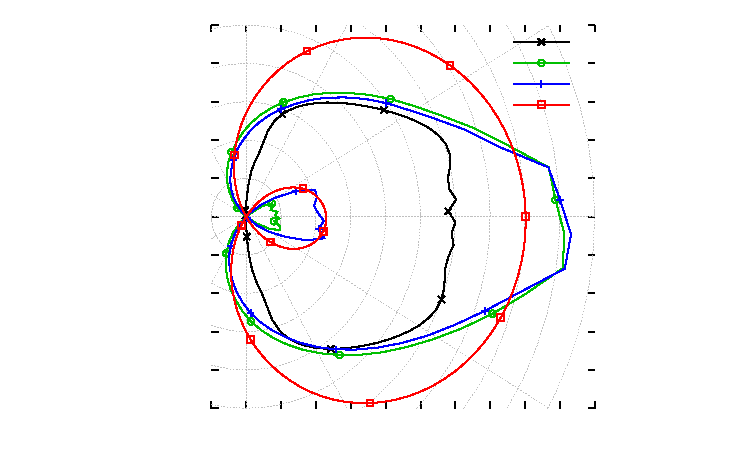
\includegraphics{/Users/seth/_thesis/figures/crashpipe2b/intens-x1-t1/intensity-x1-t1.pdf}}%
    \gplfronttext
  \end{picture}%
\endgroup

  }%
  \caption{Diffusion coefficients at $t=3$ in the flatland pipe problem.}
  \label{fig:crashaltDcoeff}
\end{figure}


%%%%%%%%%%%%%%%%%%%%%%%%%%%%%%%%%%%%%%%%%%%%%%%%%%%%%%%%%%%%%%%%%%%%%%%%%%%%%%%%
\section{2-D \texorpdfstring{``easy''}{easy} obstacle problem}
The ``easy'' obstacle problem is described in \cite{Mou2006} (and also used in
\cite{Kno2007}), where two square obstacles impede a radiation shock. In
\cite{Mou2006} the problem halts at $t=3$; for the sake of completeness we
compare the convergence of the solutions until $t=8$ in
Fig.~\ref{fig:easymkConvergence}.

\begin{figure}[htb]
  \centering
  \subfloat[Radiation temperature]{%
    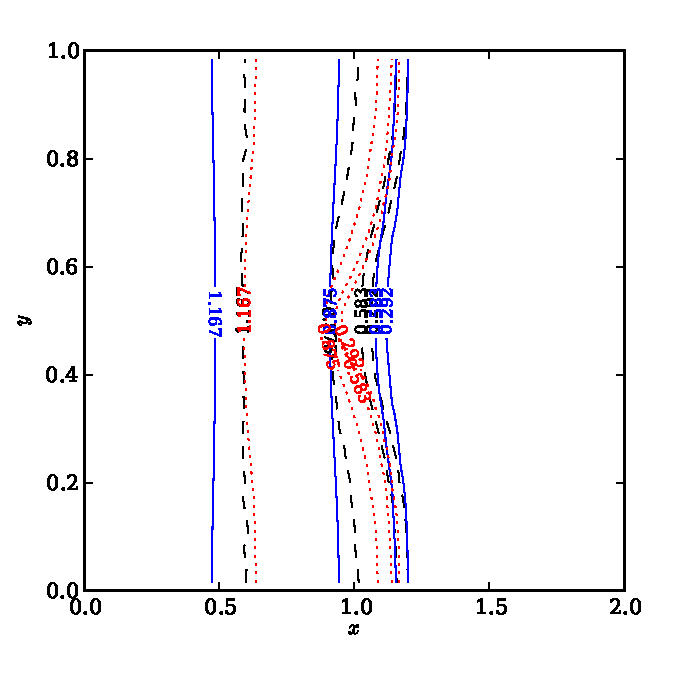
\includegraphics[width=3in]{trt_easymk/radtemp_contour_t3}
  }%
  \subfloat[Material temperature]{%
    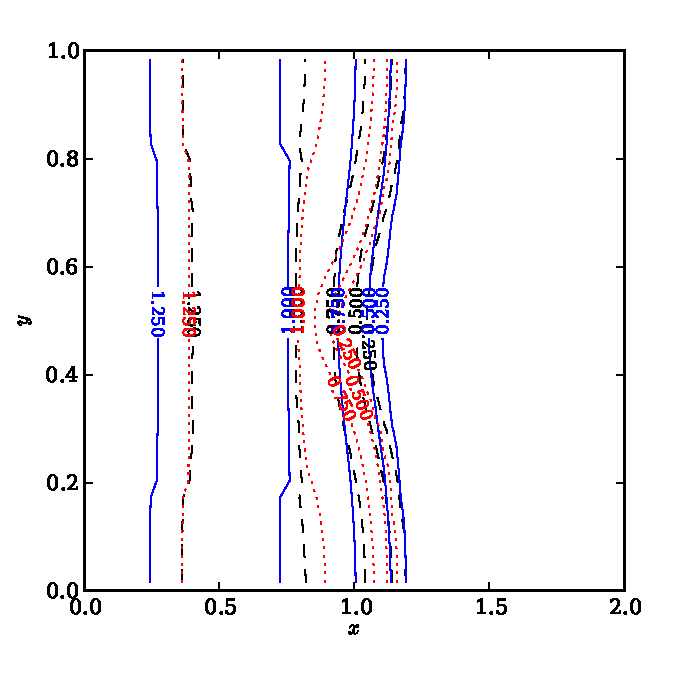
\includegraphics[width=3in]{trt_easymk/mattemp_contour_t3}
  }%
  \Caption{Contour plot of the solution at $t=3$ in the easy obstacle
  problem.}{
  The black dashed line is the IMC solution, the blue solid line is the
  FLAD solution, and the red dotted line is the FLD solution.}
  \label{fig:easymkContour}
\end{figure}

\begin{figure}[htb]
  \centering
  \subfloat[Radiation temperature]{%
    \hspace{-.25in}%
    % GNUPLOT: LaTeX picture with Postscript
\begingroup
  \makeatletter
  \providecommand\color[2][]{%
    \GenericError{(gnuplot) \space\space\space\@spaces}{%
      Package color not loaded in conjunction with
      terminal option `colourtext'%
    }{See the gnuplot documentation for explanation.%
    }{Either use 'blacktext' in gnuplot or load the package
      color.sty in LaTeX.}%
    \renewcommand\color[2][]{}%
  }%
  \providecommand\includegraphics[2][]{%
    \GenericError{(gnuplot) \space\space\space\@spaces}{%
      Package graphicx or graphics not loaded%
    }{See the gnuplot documentation for explanation.%
    }{The gnuplot epslatex terminal needs graphicx.sty or graphics.sty.}%
    \renewcommand\includegraphics[2][]{}%
  }%
  \providecommand\rotatebox[2]{#2}%
  \@ifundefined{ifGPcolor}{%
    \newif\ifGPcolor
    \GPcolortrue
  }{}%
  \@ifundefined{ifGPblacktext}{%
    \newif\ifGPblacktext
    \GPblacktexttrue
  }{}%
  % define a \g@addto@macro without @ in the name:
  \let\gplgaddtomacro\g@addto@macro
  % define empty templates for all commands taking text:
  \gdef\gplbacktext{}%
  \gdef\gplfronttext{}%
  \makeatother
  \ifGPblacktext
    % no textcolor at all
    \def\colorrgb#1{}%
    \def\colorgray#1{}%
  \else
    % gray or color?
    \ifGPcolor
      \def\colorrgb#1{\color[rgb]{#1}}%
      \def\colorgray#1{\color[gray]{#1}}%
      \expandafter\def\csname LTw\endcsname{\color{white}}%
      \expandafter\def\csname LTb\endcsname{\color{black}}%
      \expandafter\def\csname LTa\endcsname{\color{black}}%
      \expandafter\def\csname LT0\endcsname{\color[rgb]{1,0,0}}%
      \expandafter\def\csname LT1\endcsname{\color[rgb]{0,1,0}}%
      \expandafter\def\csname LT2\endcsname{\color[rgb]{0,0,1}}%
      \expandafter\def\csname LT3\endcsname{\color[rgb]{1,0,1}}%
      \expandafter\def\csname LT4\endcsname{\color[rgb]{0,1,1}}%
      \expandafter\def\csname LT5\endcsname{\color[rgb]{1,1,0}}%
      \expandafter\def\csname LT6\endcsname{\color[rgb]{0,0,0}}%
      \expandafter\def\csname LT7\endcsname{\color[rgb]{1,0.3,0}}%
      \expandafter\def\csname LT8\endcsname{\color[rgb]{0.5,0.5,0.5}}%
    \else
      % gray
      \def\colorrgb#1{\color{black}}%
      \def\colorgray#1{\color[gray]{#1}}%
      \expandafter\def\csname LTw\endcsname{\color{white}}%
      \expandafter\def\csname LTb\endcsname{\color{black}}%
      \expandafter\def\csname LTa\endcsname{\color{black}}%
      \expandafter\def\csname LT0\endcsname{\color{black}}%
      \expandafter\def\csname LT1\endcsname{\color{black}}%
      \expandafter\def\csname LT2\endcsname{\color{black}}%
      \expandafter\def\csname LT3\endcsname{\color{black}}%
      \expandafter\def\csname LT4\endcsname{\color{black}}%
      \expandafter\def\csname LT5\endcsname{\color{black}}%
      \expandafter\def\csname LT6\endcsname{\color{black}}%
      \expandafter\def\csname LT7\endcsname{\color{black}}%
      \expandafter\def\csname LT8\endcsname{\color{black}}%
    \fi
  \fi
  \setlength{\unitlength}{0.0500bp}%
  \begin{picture}(7200.00,4320.00)%
    \gplgaddtomacro\gplbacktext{%
      \csname LTb\endcsname%
      \put(1910,400){\makebox(0,0)[r]{\strut{} 0.1}}%
      \put(1910,768){\makebox(0,0)[r]{\strut{} 0.08}}%
      \put(1910,1136){\makebox(0,0)[r]{\strut{} 0.06}}%
      \put(1910,1504){\makebox(0,0)[r]{\strut{} 0.04}}%
      \put(1910,1872){\makebox(0,0)[r]{\strut{} 0.02}}%
      \put(1910,2240){\makebox(0,0)[r]{\strut{} 0}}%
      \put(1910,2607){\makebox(0,0)[r]{\strut{} 0.02}}%
      \put(1910,2975){\makebox(0,0)[r]{\strut{} 0.04}}%
      \put(1910,3343){\makebox(0,0)[r]{\strut{} 0.06}}%
      \put(1910,3711){\makebox(0,0)[r]{\strut{} 0.08}}%
      \put(1910,4079){\makebox(0,0)[r]{\strut{} 0.1}}%
      \csname LTb\endcsname%
      \put(2030,200){\makebox(0,0){\strut{} 0.02}}%
      \csname LTb\endcsname%
      \put(2364,200){\makebox(0,0){\strut{} 0}}%
      \csname LTb\endcsname%
      \put(2699,200){\makebox(0,0){\strut{} 0.02}}%
      \csname LTb\endcsname%
      \put(3033,200){\makebox(0,0){\strut{} 0.04}}%
      \csname LTb\endcsname%
      \put(3368,200){\makebox(0,0){\strut{} 0.06}}%
      \csname LTb\endcsname%
      \put(3702,200){\makebox(0,0){\strut{} 0.08}}%
      \csname LTb\endcsname%
      \put(4037,200){\makebox(0,0){\strut{} 0.1}}%
      \csname LTb\endcsname%
      \put(4371,200){\makebox(0,0){\strut{} 0.12}}%
      \csname LTb\endcsname%
      \put(4706,200){\makebox(0,0){\strut{} 0.14}}%
      \csname LTb\endcsname%
      \put(5040,200){\makebox(0,0){\strut{} 0.16}}%
      \csname LTb\endcsname%
      \put(5375,200){\makebox(0,0){\strut{} 0.18}}%
      \csname LTb\endcsname%
      \put(5709,200){\makebox(0,0){\strut{} 0.2}}%
      \csname LTb\endcsname%
      \put(1330,2239){\rotatebox{-270}{\makebox(0,0){\strut{}x1 center $(1.01,3.5)$}}}%
    }%
    \gplgaddtomacro\gplfronttext{%
      \csname LTb\endcsname%
      \put(4806,3916){\makebox(0,0)[r]{\strut{}S$_{128}$}}%
      \csname LTb\endcsname%
      \put(4806,3716){\makebox(0,0)[r]{\strut{}FLAD$_{64}$}}%
      \csname LTb\endcsname%
      \put(4806,3516){\makebox(0,0)[r]{\strut{}AD$_{64}$}}%
      \csname LTb\endcsname%
      \put(4806,3316){\makebox(0,0)[r]{\strut{}FLD}}%
    }%
    \gplbacktext
    \put(0,0){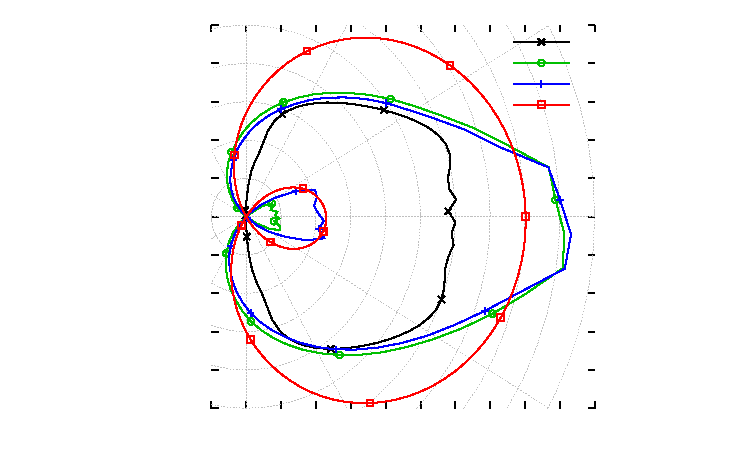
\includegraphics{/Users/seth/_thesis/figures/crashpipe2b/intens-x1-t1/intensity-x1-t1.pdf}}%
    \gplfronttext
  \end{picture}%
\endgroup

  }%
  \subfloat[Material temperature]{%
    \hspace{-.25in}%
    % GNUPLOT: LaTeX picture with Postscript
\begingroup
  \makeatletter
  \providecommand\color[2][]{%
    \GenericError{(gnuplot) \space\space\space\@spaces}{%
      Package color not loaded in conjunction with
      terminal option `colourtext'%
    }{See the gnuplot documentation for explanation.%
    }{Either use 'blacktext' in gnuplot or load the package
      color.sty in LaTeX.}%
    \renewcommand\color[2][]{}%
  }%
  \providecommand\includegraphics[2][]{%
    \GenericError{(gnuplot) \space\space\space\@spaces}{%
      Package graphicx or graphics not loaded%
    }{See the gnuplot documentation for explanation.%
    }{The gnuplot epslatex terminal needs graphicx.sty or graphics.sty.}%
    \renewcommand\includegraphics[2][]{}%
  }%
  \providecommand\rotatebox[2]{#2}%
  \@ifundefined{ifGPcolor}{%
    \newif\ifGPcolor
    \GPcolortrue
  }{}%
  \@ifundefined{ifGPblacktext}{%
    \newif\ifGPblacktext
    \GPblacktexttrue
  }{}%
  % define a \g@addto@macro without @ in the name:
  \let\gplgaddtomacro\g@addto@macro
  % define empty templates for all commands taking text:
  \gdef\gplbacktext{}%
  \gdef\gplfronttext{}%
  \makeatother
  \ifGPblacktext
    % no textcolor at all
    \def\colorrgb#1{}%
    \def\colorgray#1{}%
  \else
    % gray or color?
    \ifGPcolor
      \def\colorrgb#1{\color[rgb]{#1}}%
      \def\colorgray#1{\color[gray]{#1}}%
      \expandafter\def\csname LTw\endcsname{\color{white}}%
      \expandafter\def\csname LTb\endcsname{\color{black}}%
      \expandafter\def\csname LTa\endcsname{\color{black}}%
      \expandafter\def\csname LT0\endcsname{\color[rgb]{1,0,0}}%
      \expandafter\def\csname LT1\endcsname{\color[rgb]{0,1,0}}%
      \expandafter\def\csname LT2\endcsname{\color[rgb]{0,0,1}}%
      \expandafter\def\csname LT3\endcsname{\color[rgb]{1,0,1}}%
      \expandafter\def\csname LT4\endcsname{\color[rgb]{0,1,1}}%
      \expandafter\def\csname LT5\endcsname{\color[rgb]{1,1,0}}%
      \expandafter\def\csname LT6\endcsname{\color[rgb]{0,0,0}}%
      \expandafter\def\csname LT7\endcsname{\color[rgb]{1,0.3,0}}%
      \expandafter\def\csname LT8\endcsname{\color[rgb]{0.5,0.5,0.5}}%
    \else
      % gray
      \def\colorrgb#1{\color{black}}%
      \def\colorgray#1{\color[gray]{#1}}%
      \expandafter\def\csname LTw\endcsname{\color{white}}%
      \expandafter\def\csname LTb\endcsname{\color{black}}%
      \expandafter\def\csname LTa\endcsname{\color{black}}%
      \expandafter\def\csname LT0\endcsname{\color{black}}%
      \expandafter\def\csname LT1\endcsname{\color{black}}%
      \expandafter\def\csname LT2\endcsname{\color{black}}%
      \expandafter\def\csname LT3\endcsname{\color{black}}%
      \expandafter\def\csname LT4\endcsname{\color{black}}%
      \expandafter\def\csname LT5\endcsname{\color{black}}%
      \expandafter\def\csname LT6\endcsname{\color{black}}%
      \expandafter\def\csname LT7\endcsname{\color{black}}%
      \expandafter\def\csname LT8\endcsname{\color{black}}%
    \fi
  \fi
  \setlength{\unitlength}{0.0500bp}%
  \begin{picture}(7200.00,4320.00)%
    \gplgaddtomacro\gplbacktext{%
      \csname LTb\endcsname%
      \put(1910,400){\makebox(0,0)[r]{\strut{} 0.1}}%
      \put(1910,768){\makebox(0,0)[r]{\strut{} 0.08}}%
      \put(1910,1136){\makebox(0,0)[r]{\strut{} 0.06}}%
      \put(1910,1504){\makebox(0,0)[r]{\strut{} 0.04}}%
      \put(1910,1872){\makebox(0,0)[r]{\strut{} 0.02}}%
      \put(1910,2240){\makebox(0,0)[r]{\strut{} 0}}%
      \put(1910,2607){\makebox(0,0)[r]{\strut{} 0.02}}%
      \put(1910,2975){\makebox(0,0)[r]{\strut{} 0.04}}%
      \put(1910,3343){\makebox(0,0)[r]{\strut{} 0.06}}%
      \put(1910,3711){\makebox(0,0)[r]{\strut{} 0.08}}%
      \put(1910,4079){\makebox(0,0)[r]{\strut{} 0.1}}%
      \csname LTb\endcsname%
      \put(2030,200){\makebox(0,0){\strut{} 0.02}}%
      \csname LTb\endcsname%
      \put(2364,200){\makebox(0,0){\strut{} 0}}%
      \csname LTb\endcsname%
      \put(2699,200){\makebox(0,0){\strut{} 0.02}}%
      \csname LTb\endcsname%
      \put(3033,200){\makebox(0,0){\strut{} 0.04}}%
      \csname LTb\endcsname%
      \put(3368,200){\makebox(0,0){\strut{} 0.06}}%
      \csname LTb\endcsname%
      \put(3702,200){\makebox(0,0){\strut{} 0.08}}%
      \csname LTb\endcsname%
      \put(4037,200){\makebox(0,0){\strut{} 0.1}}%
      \csname LTb\endcsname%
      \put(4371,200){\makebox(0,0){\strut{} 0.12}}%
      \csname LTb\endcsname%
      \put(4706,200){\makebox(0,0){\strut{} 0.14}}%
      \csname LTb\endcsname%
      \put(5040,200){\makebox(0,0){\strut{} 0.16}}%
      \csname LTb\endcsname%
      \put(5375,200){\makebox(0,0){\strut{} 0.18}}%
      \csname LTb\endcsname%
      \put(5709,200){\makebox(0,0){\strut{} 0.2}}%
      \csname LTb\endcsname%
      \put(1330,2239){\rotatebox{-270}{\makebox(0,0){\strut{}x1 center $(1.01,3.5)$}}}%
    }%
    \gplgaddtomacro\gplfronttext{%
      \csname LTb\endcsname%
      \put(4806,3916){\makebox(0,0)[r]{\strut{}S$_{128}$}}%
      \csname LTb\endcsname%
      \put(4806,3716){\makebox(0,0)[r]{\strut{}FLAD$_{64}$}}%
      \csname LTb\endcsname%
      \put(4806,3516){\makebox(0,0)[r]{\strut{}AD$_{64}$}}%
      \csname LTb\endcsname%
      \put(4806,3316){\makebox(0,0)[r]{\strut{}FLD}}%
    }%
    \gplbacktext
    \put(0,0){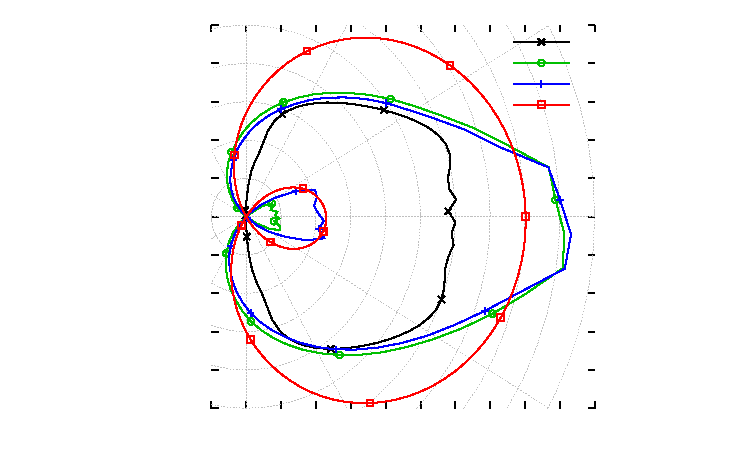
\includegraphics{/Users/seth/_thesis/figures/crashpipe2b/intens-x1-t1/intensity-x1-t1.pdf}}%
    \gplfronttext
  \end{picture}%
\endgroup

  }%
  \caption{Solution along the centerline at $t=3$ in the easy obstacle
  problem.}
  \label{fig:easymkCenterline}
\end{figure}

\begin{figure}[htb]
  \centering
  % GNUPLOT: LaTeX picture with Postscript
\begingroup
  \makeatletter
  \providecommand\color[2][]{%
    \GenericError{(gnuplot) \space\space\space\@spaces}{%
      Package color not loaded in conjunction with
      terminal option `colourtext'%
    }{See the gnuplot documentation for explanation.%
    }{Either use 'blacktext' in gnuplot or load the package
      color.sty in LaTeX.}%
    \renewcommand\color[2][]{}%
  }%
  \providecommand\includegraphics[2][]{%
    \GenericError{(gnuplot) \space\space\space\@spaces}{%
      Package graphicx or graphics not loaded%
    }{See the gnuplot documentation for explanation.%
    }{The gnuplot epslatex terminal needs graphicx.sty or graphics.sty.}%
    \renewcommand\includegraphics[2][]{}%
  }%
  \providecommand\rotatebox[2]{#2}%
  \@ifundefined{ifGPcolor}{%
    \newif\ifGPcolor
    \GPcolortrue
  }{}%
  \@ifundefined{ifGPblacktext}{%
    \newif\ifGPblacktext
    \GPblacktexttrue
  }{}%
  % define a \g@addto@macro without @ in the name:
  \let\gplgaddtomacro\g@addto@macro
  % define empty templates for all commands taking text:
  \gdef\gplbacktext{}%
  \gdef\gplfronttext{}%
  \makeatother
  \ifGPblacktext
    % no textcolor at all
    \def\colorrgb#1{}%
    \def\colorgray#1{}%
  \else
    % gray or color?
    \ifGPcolor
      \def\colorrgb#1{\color[rgb]{#1}}%
      \def\colorgray#1{\color[gray]{#1}}%
      \expandafter\def\csname LTw\endcsname{\color{white}}%
      \expandafter\def\csname LTb\endcsname{\color{black}}%
      \expandafter\def\csname LTa\endcsname{\color{black}}%
      \expandafter\def\csname LT0\endcsname{\color[rgb]{1,0,0}}%
      \expandafter\def\csname LT1\endcsname{\color[rgb]{0,1,0}}%
      \expandafter\def\csname LT2\endcsname{\color[rgb]{0,0,1}}%
      \expandafter\def\csname LT3\endcsname{\color[rgb]{1,0,1}}%
      \expandafter\def\csname LT4\endcsname{\color[rgb]{0,1,1}}%
      \expandafter\def\csname LT5\endcsname{\color[rgb]{1,1,0}}%
      \expandafter\def\csname LT6\endcsname{\color[rgb]{0,0,0}}%
      \expandafter\def\csname LT7\endcsname{\color[rgb]{1,0.3,0}}%
      \expandafter\def\csname LT8\endcsname{\color[rgb]{0.5,0.5,0.5}}%
    \else
      % gray
      \def\colorrgb#1{\color{black}}%
      \def\colorgray#1{\color[gray]{#1}}%
      \expandafter\def\csname LTw\endcsname{\color{white}}%
      \expandafter\def\csname LTb\endcsname{\color{black}}%
      \expandafter\def\csname LTa\endcsname{\color{black}}%
      \expandafter\def\csname LT0\endcsname{\color{black}}%
      \expandafter\def\csname LT1\endcsname{\color{black}}%
      \expandafter\def\csname LT2\endcsname{\color{black}}%
      \expandafter\def\csname LT3\endcsname{\color{black}}%
      \expandafter\def\csname LT4\endcsname{\color{black}}%
      \expandafter\def\csname LT5\endcsname{\color{black}}%
      \expandafter\def\csname LT6\endcsname{\color{black}}%
      \expandafter\def\csname LT7\endcsname{\color{black}}%
      \expandafter\def\csname LT8\endcsname{\color{black}}%
    \fi
  \fi
  \setlength{\unitlength}{0.0500bp}%
  \begin{picture}(7200.00,4320.00)%
    \gplgaddtomacro\gplbacktext{%
      \csname LTb\endcsname%
      \put(1910,400){\makebox(0,0)[r]{\strut{} 0.1}}%
      \put(1910,768){\makebox(0,0)[r]{\strut{} 0.08}}%
      \put(1910,1136){\makebox(0,0)[r]{\strut{} 0.06}}%
      \put(1910,1504){\makebox(0,0)[r]{\strut{} 0.04}}%
      \put(1910,1872){\makebox(0,0)[r]{\strut{} 0.02}}%
      \put(1910,2240){\makebox(0,0)[r]{\strut{} 0}}%
      \put(1910,2607){\makebox(0,0)[r]{\strut{} 0.02}}%
      \put(1910,2975){\makebox(0,0)[r]{\strut{} 0.04}}%
      \put(1910,3343){\makebox(0,0)[r]{\strut{} 0.06}}%
      \put(1910,3711){\makebox(0,0)[r]{\strut{} 0.08}}%
      \put(1910,4079){\makebox(0,0)[r]{\strut{} 0.1}}%
      \csname LTb\endcsname%
      \put(2030,200){\makebox(0,0){\strut{} 0.02}}%
      \csname LTb\endcsname%
      \put(2364,200){\makebox(0,0){\strut{} 0}}%
      \csname LTb\endcsname%
      \put(2699,200){\makebox(0,0){\strut{} 0.02}}%
      \csname LTb\endcsname%
      \put(3033,200){\makebox(0,0){\strut{} 0.04}}%
      \csname LTb\endcsname%
      \put(3368,200){\makebox(0,0){\strut{} 0.06}}%
      \csname LTb\endcsname%
      \put(3702,200){\makebox(0,0){\strut{} 0.08}}%
      \csname LTb\endcsname%
      \put(4037,200){\makebox(0,0){\strut{} 0.1}}%
      \csname LTb\endcsname%
      \put(4371,200){\makebox(0,0){\strut{} 0.12}}%
      \csname LTb\endcsname%
      \put(4706,200){\makebox(0,0){\strut{} 0.14}}%
      \csname LTb\endcsname%
      \put(5040,200){\makebox(0,0){\strut{} 0.16}}%
      \csname LTb\endcsname%
      \put(5375,200){\makebox(0,0){\strut{} 0.18}}%
      \csname LTb\endcsname%
      \put(5709,200){\makebox(0,0){\strut{} 0.2}}%
      \csname LTb\endcsname%
      \put(1330,2239){\rotatebox{-270}{\makebox(0,0){\strut{}x1 center $(1.01,3.5)$}}}%
    }%
    \gplgaddtomacro\gplfronttext{%
      \csname LTb\endcsname%
      \put(4806,3916){\makebox(0,0)[r]{\strut{}S$_{128}$}}%
      \csname LTb\endcsname%
      \put(4806,3716){\makebox(0,0)[r]{\strut{}FLAD$_{64}$}}%
      \csname LTb\endcsname%
      \put(4806,3516){\makebox(0,0)[r]{\strut{}AD$_{64}$}}%
      \csname LTb\endcsname%
      \put(4806,3316){\makebox(0,0)[r]{\strut{}FLD}}%
    }%
    \gplbacktext
    \put(0,0){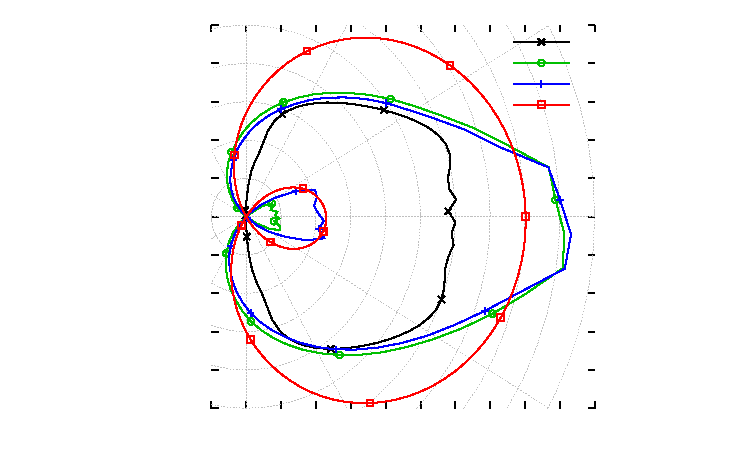
\includegraphics{/Users/seth/_thesis/figures/crashpipe2b/intens-x1-t1/intensity-x1-t1.pdf}}%
    \gplfronttext
  \end{picture}%
\endgroup

  \caption{Relative difference of the material temperature in the easy obstacle
  problem.}
  \label{fig:easymkConvergence}
\end{figure}

%%%%%%%%%%%%%%%%%%%%%%%%%%%%%%%%%%%%%%%%%%%%%%%%%%%%%%%%%%%%%%%%%%%%%%%%%%%%%%%%
\section{2-D \texorpdfstring{``hard''}{hard} obstacle problem}

\begin{figure}[htb]
  \centering
  % GNUPLOT: LaTeX picture with Postscript
\begingroup
  \makeatletter
  \providecommand\color[2][]{%
    \GenericError{(gnuplot) \space\space\space\@spaces}{%
      Package color not loaded in conjunction with
      terminal option `colourtext'%
    }{See the gnuplot documentation for explanation.%
    }{Either use 'blacktext' in gnuplot or load the package
      color.sty in LaTeX.}%
    \renewcommand\color[2][]{}%
  }%
  \providecommand\includegraphics[2][]{%
    \GenericError{(gnuplot) \space\space\space\@spaces}{%
      Package graphicx or graphics not loaded%
    }{See the gnuplot documentation for explanation.%
    }{The gnuplot epslatex terminal needs graphicx.sty or graphics.sty.}%
    \renewcommand\includegraphics[2][]{}%
  }%
  \providecommand\rotatebox[2]{#2}%
  \@ifundefined{ifGPcolor}{%
    \newif\ifGPcolor
    \GPcolortrue
  }{}%
  \@ifundefined{ifGPblacktext}{%
    \newif\ifGPblacktext
    \GPblacktexttrue
  }{}%
  % define a \g@addto@macro without @ in the name:
  \let\gplgaddtomacro\g@addto@macro
  % define empty templates for all commands taking text:
  \gdef\gplbacktext{}%
  \gdef\gplfronttext{}%
  \makeatother
  \ifGPblacktext
    % no textcolor at all
    \def\colorrgb#1{}%
    \def\colorgray#1{}%
  \else
    % gray or color?
    \ifGPcolor
      \def\colorrgb#1{\color[rgb]{#1}}%
      \def\colorgray#1{\color[gray]{#1}}%
      \expandafter\def\csname LTw\endcsname{\color{white}}%
      \expandafter\def\csname LTb\endcsname{\color{black}}%
      \expandafter\def\csname LTa\endcsname{\color{black}}%
      \expandafter\def\csname LT0\endcsname{\color[rgb]{1,0,0}}%
      \expandafter\def\csname LT1\endcsname{\color[rgb]{0,1,0}}%
      \expandafter\def\csname LT2\endcsname{\color[rgb]{0,0,1}}%
      \expandafter\def\csname LT3\endcsname{\color[rgb]{1,0,1}}%
      \expandafter\def\csname LT4\endcsname{\color[rgb]{0,1,1}}%
      \expandafter\def\csname LT5\endcsname{\color[rgb]{1,1,0}}%
      \expandafter\def\csname LT6\endcsname{\color[rgb]{0,0,0}}%
      \expandafter\def\csname LT7\endcsname{\color[rgb]{1,0.3,0}}%
      \expandafter\def\csname LT8\endcsname{\color[rgb]{0.5,0.5,0.5}}%
    \else
      % gray
      \def\colorrgb#1{\color{black}}%
      \def\colorgray#1{\color[gray]{#1}}%
      \expandafter\def\csname LTw\endcsname{\color{white}}%
      \expandafter\def\csname LTb\endcsname{\color{black}}%
      \expandafter\def\csname LTa\endcsname{\color{black}}%
      \expandafter\def\csname LT0\endcsname{\color{black}}%
      \expandafter\def\csname LT1\endcsname{\color{black}}%
      \expandafter\def\csname LT2\endcsname{\color{black}}%
      \expandafter\def\csname LT3\endcsname{\color{black}}%
      \expandafter\def\csname LT4\endcsname{\color{black}}%
      \expandafter\def\csname LT5\endcsname{\color{black}}%
      \expandafter\def\csname LT6\endcsname{\color{black}}%
      \expandafter\def\csname LT7\endcsname{\color{black}}%
      \expandafter\def\csname LT8\endcsname{\color{black}}%
    \fi
  \fi
  \setlength{\unitlength}{0.0500bp}%
  \begin{picture}(7200.00,4320.00)%
    \gplgaddtomacro\gplbacktext{%
      \csname LTb\endcsname%
      \put(1910,400){\makebox(0,0)[r]{\strut{} 0.1}}%
      \put(1910,768){\makebox(0,0)[r]{\strut{} 0.08}}%
      \put(1910,1136){\makebox(0,0)[r]{\strut{} 0.06}}%
      \put(1910,1504){\makebox(0,0)[r]{\strut{} 0.04}}%
      \put(1910,1872){\makebox(0,0)[r]{\strut{} 0.02}}%
      \put(1910,2240){\makebox(0,0)[r]{\strut{} 0}}%
      \put(1910,2607){\makebox(0,0)[r]{\strut{} 0.02}}%
      \put(1910,2975){\makebox(0,0)[r]{\strut{} 0.04}}%
      \put(1910,3343){\makebox(0,0)[r]{\strut{} 0.06}}%
      \put(1910,3711){\makebox(0,0)[r]{\strut{} 0.08}}%
      \put(1910,4079){\makebox(0,0)[r]{\strut{} 0.1}}%
      \csname LTb\endcsname%
      \put(2030,200){\makebox(0,0){\strut{} 0.02}}%
      \csname LTb\endcsname%
      \put(2364,200){\makebox(0,0){\strut{} 0}}%
      \csname LTb\endcsname%
      \put(2699,200){\makebox(0,0){\strut{} 0.02}}%
      \csname LTb\endcsname%
      \put(3033,200){\makebox(0,0){\strut{} 0.04}}%
      \csname LTb\endcsname%
      \put(3368,200){\makebox(0,0){\strut{} 0.06}}%
      \csname LTb\endcsname%
      \put(3702,200){\makebox(0,0){\strut{} 0.08}}%
      \csname LTb\endcsname%
      \put(4037,200){\makebox(0,0){\strut{} 0.1}}%
      \csname LTb\endcsname%
      \put(4371,200){\makebox(0,0){\strut{} 0.12}}%
      \csname LTb\endcsname%
      \put(4706,200){\makebox(0,0){\strut{} 0.14}}%
      \csname LTb\endcsname%
      \put(5040,200){\makebox(0,0){\strut{} 0.16}}%
      \csname LTb\endcsname%
      \put(5375,200){\makebox(0,0){\strut{} 0.18}}%
      \csname LTb\endcsname%
      \put(5709,200){\makebox(0,0){\strut{} 0.2}}%
      \csname LTb\endcsname%
      \put(1330,2239){\rotatebox{-270}{\makebox(0,0){\strut{}x1 center $(1.01,3.5)$}}}%
    }%
    \gplgaddtomacro\gplfronttext{%
      \csname LTb\endcsname%
      \put(4806,3916){\makebox(0,0)[r]{\strut{}S$_{128}$}}%
      \csname LTb\endcsname%
      \put(4806,3716){\makebox(0,0)[r]{\strut{}FLAD$_{64}$}}%
      \csname LTb\endcsname%
      \put(4806,3516){\makebox(0,0)[r]{\strut{}AD$_{64}$}}%
      \csname LTb\endcsname%
      \put(4806,3316){\makebox(0,0)[r]{\strut{}FLD}}%
    }%
    \gplbacktext
    \put(0,0){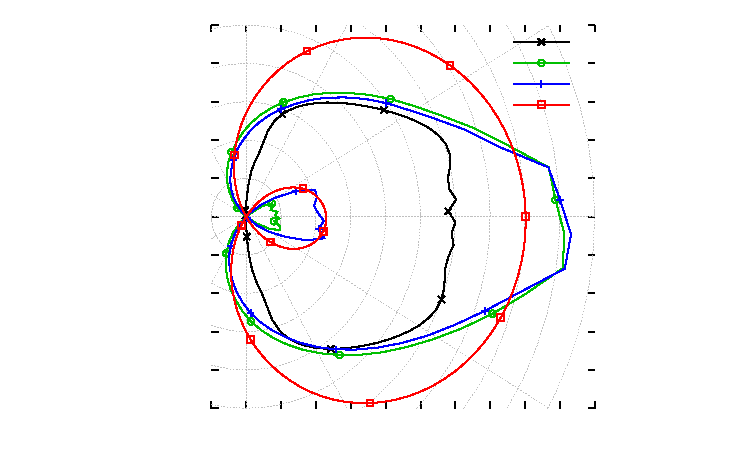
\includegraphics{/Users/seth/_thesis/figures/crashpipe2b/intens-x1-t1/intensity-x1-t1.pdf}}%
    \gplfronttext
  \end{picture}%
\endgroup

  \caption{Wavefront plot along the diagonal in the hard obstacle problem.}
  \label{fig:hardmkContour}
\end{figure}

\begin{figure}[htb]
  \centering
  \subfloat[Radiation temperature]{%
    \hspace{-.25in}%
    % GNUPLOT: LaTeX picture with Postscript
\begingroup
  \makeatletter
  \providecommand\color[2][]{%
    \GenericError{(gnuplot) \space\space\space\@spaces}{%
      Package color not loaded in conjunction with
      terminal option `colourtext'%
    }{See the gnuplot documentation for explanation.%
    }{Either use 'blacktext' in gnuplot or load the package
      color.sty in LaTeX.}%
    \renewcommand\color[2][]{}%
  }%
  \providecommand\includegraphics[2][]{%
    \GenericError{(gnuplot) \space\space\space\@spaces}{%
      Package graphicx or graphics not loaded%
    }{See the gnuplot documentation for explanation.%
    }{The gnuplot epslatex terminal needs graphicx.sty or graphics.sty.}%
    \renewcommand\includegraphics[2][]{}%
  }%
  \providecommand\rotatebox[2]{#2}%
  \@ifundefined{ifGPcolor}{%
    \newif\ifGPcolor
    \GPcolortrue
  }{}%
  \@ifundefined{ifGPblacktext}{%
    \newif\ifGPblacktext
    \GPblacktexttrue
  }{}%
  % define a \g@addto@macro without @ in the name:
  \let\gplgaddtomacro\g@addto@macro
  % define empty templates for all commands taking text:
  \gdef\gplbacktext{}%
  \gdef\gplfronttext{}%
  \makeatother
  \ifGPblacktext
    % no textcolor at all
    \def\colorrgb#1{}%
    \def\colorgray#1{}%
  \else
    % gray or color?
    \ifGPcolor
      \def\colorrgb#1{\color[rgb]{#1}}%
      \def\colorgray#1{\color[gray]{#1}}%
      \expandafter\def\csname LTw\endcsname{\color{white}}%
      \expandafter\def\csname LTb\endcsname{\color{black}}%
      \expandafter\def\csname LTa\endcsname{\color{black}}%
      \expandafter\def\csname LT0\endcsname{\color[rgb]{1,0,0}}%
      \expandafter\def\csname LT1\endcsname{\color[rgb]{0,1,0}}%
      \expandafter\def\csname LT2\endcsname{\color[rgb]{0,0,1}}%
      \expandafter\def\csname LT3\endcsname{\color[rgb]{1,0,1}}%
      \expandafter\def\csname LT4\endcsname{\color[rgb]{0,1,1}}%
      \expandafter\def\csname LT5\endcsname{\color[rgb]{1,1,0}}%
      \expandafter\def\csname LT6\endcsname{\color[rgb]{0,0,0}}%
      \expandafter\def\csname LT7\endcsname{\color[rgb]{1,0.3,0}}%
      \expandafter\def\csname LT8\endcsname{\color[rgb]{0.5,0.5,0.5}}%
    \else
      % gray
      \def\colorrgb#1{\color{black}}%
      \def\colorgray#1{\color[gray]{#1}}%
      \expandafter\def\csname LTw\endcsname{\color{white}}%
      \expandafter\def\csname LTb\endcsname{\color{black}}%
      \expandafter\def\csname LTa\endcsname{\color{black}}%
      \expandafter\def\csname LT0\endcsname{\color{black}}%
      \expandafter\def\csname LT1\endcsname{\color{black}}%
      \expandafter\def\csname LT2\endcsname{\color{black}}%
      \expandafter\def\csname LT3\endcsname{\color{black}}%
      \expandafter\def\csname LT4\endcsname{\color{black}}%
      \expandafter\def\csname LT5\endcsname{\color{black}}%
      \expandafter\def\csname LT6\endcsname{\color{black}}%
      \expandafter\def\csname LT7\endcsname{\color{black}}%
      \expandafter\def\csname LT8\endcsname{\color{black}}%
    \fi
  \fi
  \setlength{\unitlength}{0.0500bp}%
  \begin{picture}(7200.00,4320.00)%
    \gplgaddtomacro\gplbacktext{%
      \csname LTb\endcsname%
      \put(1910,400){\makebox(0,0)[r]{\strut{} 0.1}}%
      \put(1910,768){\makebox(0,0)[r]{\strut{} 0.08}}%
      \put(1910,1136){\makebox(0,0)[r]{\strut{} 0.06}}%
      \put(1910,1504){\makebox(0,0)[r]{\strut{} 0.04}}%
      \put(1910,1872){\makebox(0,0)[r]{\strut{} 0.02}}%
      \put(1910,2240){\makebox(0,0)[r]{\strut{} 0}}%
      \put(1910,2607){\makebox(0,0)[r]{\strut{} 0.02}}%
      \put(1910,2975){\makebox(0,0)[r]{\strut{} 0.04}}%
      \put(1910,3343){\makebox(0,0)[r]{\strut{} 0.06}}%
      \put(1910,3711){\makebox(0,0)[r]{\strut{} 0.08}}%
      \put(1910,4079){\makebox(0,0)[r]{\strut{} 0.1}}%
      \csname LTb\endcsname%
      \put(2030,200){\makebox(0,0){\strut{} 0.02}}%
      \csname LTb\endcsname%
      \put(2364,200){\makebox(0,0){\strut{} 0}}%
      \csname LTb\endcsname%
      \put(2699,200){\makebox(0,0){\strut{} 0.02}}%
      \csname LTb\endcsname%
      \put(3033,200){\makebox(0,0){\strut{} 0.04}}%
      \csname LTb\endcsname%
      \put(3368,200){\makebox(0,0){\strut{} 0.06}}%
      \csname LTb\endcsname%
      \put(3702,200){\makebox(0,0){\strut{} 0.08}}%
      \csname LTb\endcsname%
      \put(4037,200){\makebox(0,0){\strut{} 0.1}}%
      \csname LTb\endcsname%
      \put(4371,200){\makebox(0,0){\strut{} 0.12}}%
      \csname LTb\endcsname%
      \put(4706,200){\makebox(0,0){\strut{} 0.14}}%
      \csname LTb\endcsname%
      \put(5040,200){\makebox(0,0){\strut{} 0.16}}%
      \csname LTb\endcsname%
      \put(5375,200){\makebox(0,0){\strut{} 0.18}}%
      \csname LTb\endcsname%
      \put(5709,200){\makebox(0,0){\strut{} 0.2}}%
      \csname LTb\endcsname%
      \put(1330,2239){\rotatebox{-270}{\makebox(0,0){\strut{}x1 center $(1.01,3.5)$}}}%
    }%
    \gplgaddtomacro\gplfronttext{%
      \csname LTb\endcsname%
      \put(4806,3916){\makebox(0,0)[r]{\strut{}S$_{128}$}}%
      \csname LTb\endcsname%
      \put(4806,3716){\makebox(0,0)[r]{\strut{}FLAD$_{64}$}}%
      \csname LTb\endcsname%
      \put(4806,3516){\makebox(0,0)[r]{\strut{}AD$_{64}$}}%
      \csname LTb\endcsname%
      \put(4806,3316){\makebox(0,0)[r]{\strut{}FLD}}%
    }%
    \gplbacktext
    \put(0,0){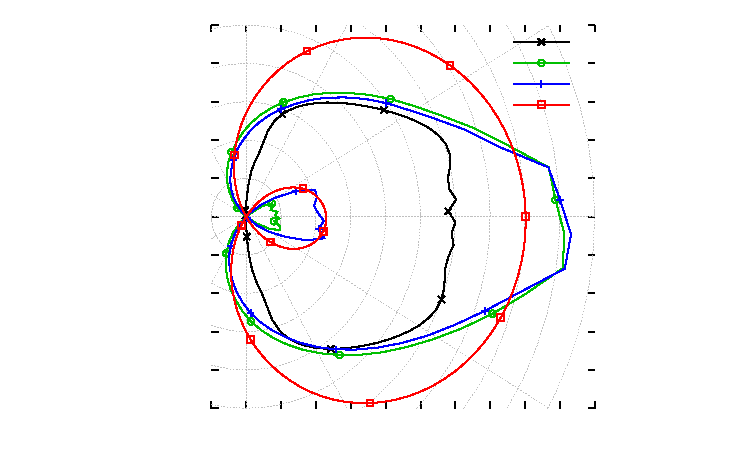
\includegraphics{/Users/seth/_thesis/figures/crashpipe2b/intens-x1-t1/intensity-x1-t1.pdf}}%
    \gplfronttext
  \end{picture}%
\endgroup

  }%
  \subfloat[Material temperature]{%
    \hspace{-.25in}%
    % GNUPLOT: LaTeX picture with Postscript
\begingroup
  \makeatletter
  \providecommand\color[2][]{%
    \GenericError{(gnuplot) \space\space\space\@spaces}{%
      Package color not loaded in conjunction with
      terminal option `colourtext'%
    }{See the gnuplot documentation for explanation.%
    }{Either use 'blacktext' in gnuplot or load the package
      color.sty in LaTeX.}%
    \renewcommand\color[2][]{}%
  }%
  \providecommand\includegraphics[2][]{%
    \GenericError{(gnuplot) \space\space\space\@spaces}{%
      Package graphicx or graphics not loaded%
    }{See the gnuplot documentation for explanation.%
    }{The gnuplot epslatex terminal needs graphicx.sty or graphics.sty.}%
    \renewcommand\includegraphics[2][]{}%
  }%
  \providecommand\rotatebox[2]{#2}%
  \@ifundefined{ifGPcolor}{%
    \newif\ifGPcolor
    \GPcolortrue
  }{}%
  \@ifundefined{ifGPblacktext}{%
    \newif\ifGPblacktext
    \GPblacktexttrue
  }{}%
  % define a \g@addto@macro without @ in the name:
  \let\gplgaddtomacro\g@addto@macro
  % define empty templates for all commands taking text:
  \gdef\gplbacktext{}%
  \gdef\gplfronttext{}%
  \makeatother
  \ifGPblacktext
    % no textcolor at all
    \def\colorrgb#1{}%
    \def\colorgray#1{}%
  \else
    % gray or color?
    \ifGPcolor
      \def\colorrgb#1{\color[rgb]{#1}}%
      \def\colorgray#1{\color[gray]{#1}}%
      \expandafter\def\csname LTw\endcsname{\color{white}}%
      \expandafter\def\csname LTb\endcsname{\color{black}}%
      \expandafter\def\csname LTa\endcsname{\color{black}}%
      \expandafter\def\csname LT0\endcsname{\color[rgb]{1,0,0}}%
      \expandafter\def\csname LT1\endcsname{\color[rgb]{0,1,0}}%
      \expandafter\def\csname LT2\endcsname{\color[rgb]{0,0,1}}%
      \expandafter\def\csname LT3\endcsname{\color[rgb]{1,0,1}}%
      \expandafter\def\csname LT4\endcsname{\color[rgb]{0,1,1}}%
      \expandafter\def\csname LT5\endcsname{\color[rgb]{1,1,0}}%
      \expandafter\def\csname LT6\endcsname{\color[rgb]{0,0,0}}%
      \expandafter\def\csname LT7\endcsname{\color[rgb]{1,0.3,0}}%
      \expandafter\def\csname LT8\endcsname{\color[rgb]{0.5,0.5,0.5}}%
    \else
      % gray
      \def\colorrgb#1{\color{black}}%
      \def\colorgray#1{\color[gray]{#1}}%
      \expandafter\def\csname LTw\endcsname{\color{white}}%
      \expandafter\def\csname LTb\endcsname{\color{black}}%
      \expandafter\def\csname LTa\endcsname{\color{black}}%
      \expandafter\def\csname LT0\endcsname{\color{black}}%
      \expandafter\def\csname LT1\endcsname{\color{black}}%
      \expandafter\def\csname LT2\endcsname{\color{black}}%
      \expandafter\def\csname LT3\endcsname{\color{black}}%
      \expandafter\def\csname LT4\endcsname{\color{black}}%
      \expandafter\def\csname LT5\endcsname{\color{black}}%
      \expandafter\def\csname LT6\endcsname{\color{black}}%
      \expandafter\def\csname LT7\endcsname{\color{black}}%
      \expandafter\def\csname LT8\endcsname{\color{black}}%
    \fi
  \fi
  \setlength{\unitlength}{0.0500bp}%
  \begin{picture}(7200.00,4320.00)%
    \gplgaddtomacro\gplbacktext{%
      \csname LTb\endcsname%
      \put(1910,400){\makebox(0,0)[r]{\strut{} 0.1}}%
      \put(1910,768){\makebox(0,0)[r]{\strut{} 0.08}}%
      \put(1910,1136){\makebox(0,0)[r]{\strut{} 0.06}}%
      \put(1910,1504){\makebox(0,0)[r]{\strut{} 0.04}}%
      \put(1910,1872){\makebox(0,0)[r]{\strut{} 0.02}}%
      \put(1910,2240){\makebox(0,0)[r]{\strut{} 0}}%
      \put(1910,2607){\makebox(0,0)[r]{\strut{} 0.02}}%
      \put(1910,2975){\makebox(0,0)[r]{\strut{} 0.04}}%
      \put(1910,3343){\makebox(0,0)[r]{\strut{} 0.06}}%
      \put(1910,3711){\makebox(0,0)[r]{\strut{} 0.08}}%
      \put(1910,4079){\makebox(0,0)[r]{\strut{} 0.1}}%
      \csname LTb\endcsname%
      \put(2030,200){\makebox(0,0){\strut{} 0.02}}%
      \csname LTb\endcsname%
      \put(2364,200){\makebox(0,0){\strut{} 0}}%
      \csname LTb\endcsname%
      \put(2699,200){\makebox(0,0){\strut{} 0.02}}%
      \csname LTb\endcsname%
      \put(3033,200){\makebox(0,0){\strut{} 0.04}}%
      \csname LTb\endcsname%
      \put(3368,200){\makebox(0,0){\strut{} 0.06}}%
      \csname LTb\endcsname%
      \put(3702,200){\makebox(0,0){\strut{} 0.08}}%
      \csname LTb\endcsname%
      \put(4037,200){\makebox(0,0){\strut{} 0.1}}%
      \csname LTb\endcsname%
      \put(4371,200){\makebox(0,0){\strut{} 0.12}}%
      \csname LTb\endcsname%
      \put(4706,200){\makebox(0,0){\strut{} 0.14}}%
      \csname LTb\endcsname%
      \put(5040,200){\makebox(0,0){\strut{} 0.16}}%
      \csname LTb\endcsname%
      \put(5375,200){\makebox(0,0){\strut{} 0.18}}%
      \csname LTb\endcsname%
      \put(5709,200){\makebox(0,0){\strut{} 0.2}}%
      \csname LTb\endcsname%
      \put(1330,2239){\rotatebox{-270}{\makebox(0,0){\strut{}x1 center $(1.01,3.5)$}}}%
    }%
    \gplgaddtomacro\gplfronttext{%
      \csname LTb\endcsname%
      \put(4806,3916){\makebox(0,0)[r]{\strut{}S$_{128}$}}%
      \csname LTb\endcsname%
      \put(4806,3716){\makebox(0,0)[r]{\strut{}FLAD$_{64}$}}%
      \csname LTb\endcsname%
      \put(4806,3516){\makebox(0,0)[r]{\strut{}AD$_{64}$}}%
      \csname LTb\endcsname%
      \put(4806,3316){\makebox(0,0)[r]{\strut{}FLD}}%
    }%
    \gplbacktext
    \put(0,0){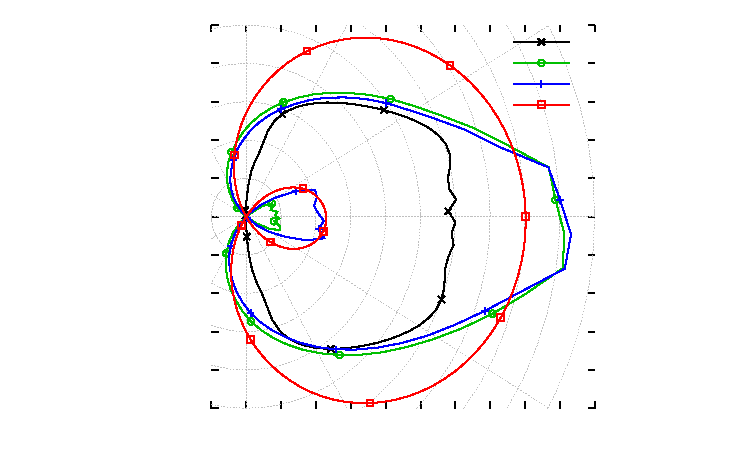
\includegraphics{/Users/seth/_thesis/figures/crashpipe2b/intens-x1-t1/intensity-x1-t1.pdf}}%
    \gplfronttext
  \end{picture}%
\endgroup

  }%
  \caption{Solution along the diagonal at $t=3$ in the hard obstacle problem.}
  \label{fig:hardmkCenterline}
\end{figure}

\begin{figure}[htb]
  \centering
  \hspace{-1in}%
  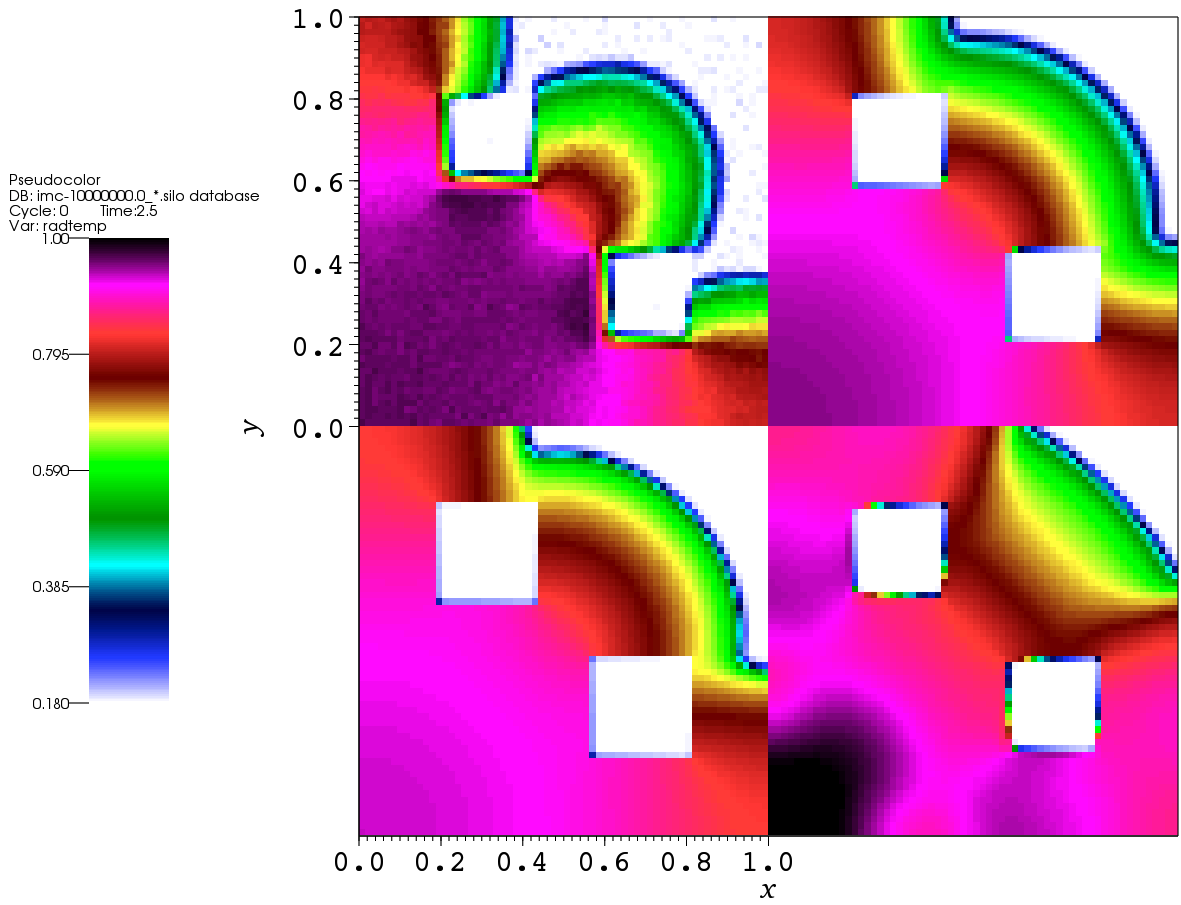
\includegraphics[width=4in]{trt_hardmk/radtemp_t25}
  \Caption{Pseudocolor plots of the radiation temperature at $t=2.5$.}{
  Clockwise from upper left: IMC, FLAD, AP1, FLD.}
  \label{fig:hardmkConvergence}
\end{figure}

%%%%%%%%%%%%%%%%%%%%%%%%%%%%%%%%%%%%%%%%%%%%%%%%%%%%%%%%%%%%%%%%%%%%%%%%%%%%%%%%
\clearpage
\section{CRASH problem}
The profile of energy deposition in the wall is an important diagnostic in the
radiation hydrodynamics problem relevant to the CRASH program \cite{HolCom2011}.

The physical opacities in Fig.~\ref{fig:seriousOpacity} are interpolated from a
table of Rosseland opacities given as $\sigma(\log \rho, \log T)$, 
%
\begin{figure}[htb]
  \centering\small
  % GNUPLOT: LaTeX picture with Postscript
\begingroup
  \makeatletter
  \providecommand\color[2][]{%
    \GenericError{(gnuplot) \space\space\space\@spaces}{%
      Package color not loaded in conjunction with
      terminal option `colourtext'%
    }{See the gnuplot documentation for explanation.%
    }{Either use 'blacktext' in gnuplot or load the package
      color.sty in LaTeX.}%
    \renewcommand\color[2][]{}%
  }%
  \providecommand\includegraphics[2][]{%
    \GenericError{(gnuplot) \space\space\space\@spaces}{%
      Package graphicx or graphics not loaded%
    }{See the gnuplot documentation for explanation.%
    }{The gnuplot epslatex terminal needs graphicx.sty or graphics.sty.}%
    \renewcommand\includegraphics[2][]{}%
  }%
  \providecommand\rotatebox[2]{#2}%
  \@ifundefined{ifGPcolor}{%
    \newif\ifGPcolor
    \GPcolortrue
  }{}%
  \@ifundefined{ifGPblacktext}{%
    \newif\ifGPblacktext
    \GPblacktexttrue
  }{}%
  % define a \g@addto@macro without @ in the name:
  \let\gplgaddtomacro\g@addto@macro
  % define empty templates for all commands taking text:
  \gdef\gplbacktext{}%
  \gdef\gplfronttext{}%
  \makeatother
  \ifGPblacktext
    % no textcolor at all
    \def\colorrgb#1{}%
    \def\colorgray#1{}%
  \else
    % gray or color?
    \ifGPcolor
      \def\colorrgb#1{\color[rgb]{#1}}%
      \def\colorgray#1{\color[gray]{#1}}%
      \expandafter\def\csname LTw\endcsname{\color{white}}%
      \expandafter\def\csname LTb\endcsname{\color{black}}%
      \expandafter\def\csname LTa\endcsname{\color{black}}%
      \expandafter\def\csname LT0\endcsname{\color[rgb]{1,0,0}}%
      \expandafter\def\csname LT1\endcsname{\color[rgb]{0,1,0}}%
      \expandafter\def\csname LT2\endcsname{\color[rgb]{0,0,1}}%
      \expandafter\def\csname LT3\endcsname{\color[rgb]{1,0,1}}%
      \expandafter\def\csname LT4\endcsname{\color[rgb]{0,1,1}}%
      \expandafter\def\csname LT5\endcsname{\color[rgb]{1,1,0}}%
      \expandafter\def\csname LT6\endcsname{\color[rgb]{0,0,0}}%
      \expandafter\def\csname LT7\endcsname{\color[rgb]{1,0.3,0}}%
      \expandafter\def\csname LT8\endcsname{\color[rgb]{0.5,0.5,0.5}}%
    \else
      % gray
      \def\colorrgb#1{\color{black}}%
      \def\colorgray#1{\color[gray]{#1}}%
      \expandafter\def\csname LTw\endcsname{\color{white}}%
      \expandafter\def\csname LTb\endcsname{\color{black}}%
      \expandafter\def\csname LTa\endcsname{\color{black}}%
      \expandafter\def\csname LT0\endcsname{\color{black}}%
      \expandafter\def\csname LT1\endcsname{\color{black}}%
      \expandafter\def\csname LT2\endcsname{\color{black}}%
      \expandafter\def\csname LT3\endcsname{\color{black}}%
      \expandafter\def\csname LT4\endcsname{\color{black}}%
      \expandafter\def\csname LT5\endcsname{\color{black}}%
      \expandafter\def\csname LT6\endcsname{\color{black}}%
      \expandafter\def\csname LT7\endcsname{\color{black}}%
      \expandafter\def\csname LT8\endcsname{\color{black}}%
    \fi
  \fi
  \setlength{\unitlength}{0.0500bp}%
  \begin{picture}(7200.00,4320.00)%
    \gplgaddtomacro\gplbacktext{%
      \csname LTb\endcsname%
      \put(1910,400){\makebox(0,0)[r]{\strut{} 0.1}}%
      \put(1910,768){\makebox(0,0)[r]{\strut{} 0.08}}%
      \put(1910,1136){\makebox(0,0)[r]{\strut{} 0.06}}%
      \put(1910,1504){\makebox(0,0)[r]{\strut{} 0.04}}%
      \put(1910,1872){\makebox(0,0)[r]{\strut{} 0.02}}%
      \put(1910,2240){\makebox(0,0)[r]{\strut{} 0}}%
      \put(1910,2607){\makebox(0,0)[r]{\strut{} 0.02}}%
      \put(1910,2975){\makebox(0,0)[r]{\strut{} 0.04}}%
      \put(1910,3343){\makebox(0,0)[r]{\strut{} 0.06}}%
      \put(1910,3711){\makebox(0,0)[r]{\strut{} 0.08}}%
      \put(1910,4079){\makebox(0,0)[r]{\strut{} 0.1}}%
      \csname LTb\endcsname%
      \put(2030,200){\makebox(0,0){\strut{} 0.02}}%
      \csname LTb\endcsname%
      \put(2364,200){\makebox(0,0){\strut{} 0}}%
      \csname LTb\endcsname%
      \put(2699,200){\makebox(0,0){\strut{} 0.02}}%
      \csname LTb\endcsname%
      \put(3033,200){\makebox(0,0){\strut{} 0.04}}%
      \csname LTb\endcsname%
      \put(3368,200){\makebox(0,0){\strut{} 0.06}}%
      \csname LTb\endcsname%
      \put(3702,200){\makebox(0,0){\strut{} 0.08}}%
      \csname LTb\endcsname%
      \put(4037,200){\makebox(0,0){\strut{} 0.1}}%
      \csname LTb\endcsname%
      \put(4371,200){\makebox(0,0){\strut{} 0.12}}%
      \csname LTb\endcsname%
      \put(4706,200){\makebox(0,0){\strut{} 0.14}}%
      \csname LTb\endcsname%
      \put(5040,200){\makebox(0,0){\strut{} 0.16}}%
      \csname LTb\endcsname%
      \put(5375,200){\makebox(0,0){\strut{} 0.18}}%
      \csname LTb\endcsname%
      \put(5709,200){\makebox(0,0){\strut{} 0.2}}%
      \csname LTb\endcsname%
      \put(1330,2239){\rotatebox{-270}{\makebox(0,0){\strut{}x1 center $(1.01,3.5)$}}}%
    }%
    \gplgaddtomacro\gplfronttext{%
      \csname LTb\endcsname%
      \put(4806,3916){\makebox(0,0)[r]{\strut{}S$_{128}$}}%
      \csname LTb\endcsname%
      \put(4806,3716){\makebox(0,0)[r]{\strut{}FLAD$_{64}$}}%
      \csname LTb\endcsname%
      \put(4806,3516){\makebox(0,0)[r]{\strut{}AD$_{64}$}}%
      \csname LTb\endcsname%
      \put(4806,3316){\makebox(0,0)[r]{\strut{}FLD}}%
    }%
    \gplbacktext
    \put(0,0){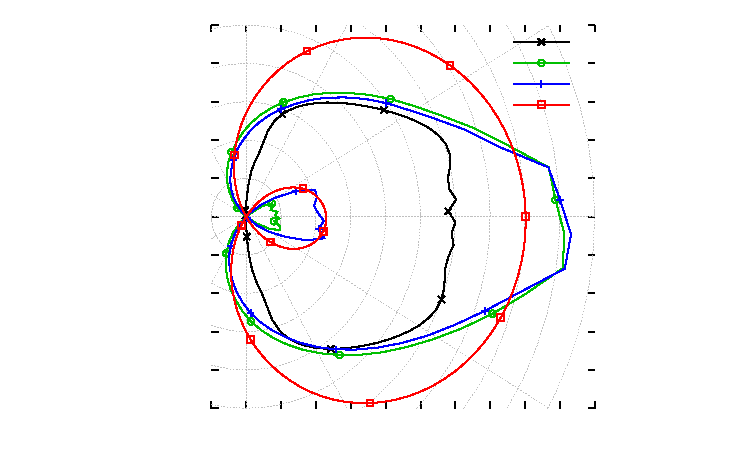
\includegraphics{/Users/seth/_thesis/figures/crashpipe2b/intens-x1-t1/intensity-x1-t1.pdf}}%
    \gplfronttext
  \end{picture}%
\endgroup

  \Caption{True opacities and modeled versions used in the CRASH simulation
  problem.}{
  The true opacities (solid line) are generated from physical data,
  and the model opacities (dashed lines of the same color and marker) are
  fitted.}
  \label{fig:seriousOpacity}
\end{figure}
%
and a crude temperature model approximates the more realistic model:
\begin{equation*}
  \sigma(T;\gamma,T_1,T_2) =
  \begin{cases}
    \gamma   & T < T_1\,, \\
    \gamma \left( \frac{T}{T_1} \right)^{-3}   & T_1 \le T < T_2\,, \\
    \gamma \left( \frac{T_2}{T_1} \right)^{-3}
    \left( \frac{T}{T_2} \right)^{-1/2}   & T_2 \le T \,.
  \end{cases}
\end{equation*}

The values for $\gamma$, $T_1$, and $T_2$, along with other physical properties
of the materials, are given in Table~\ref{tab:seriousPhysics}.
\begin{table}[htb]
  \centering
  \begin{tabular}{llllll}
\toprule
 Material & Width & $c_v$ & $\gamma$ & $T_1$ & $T_2$
\\ \midrule
Plastic (original) & 0.0025 & $1.89\EE{23}$ & $14500$ & $80$ & $2.3\EE3$\\
Plastic (stretched) & 0.01 & $4.73\EE{22}$ & $3620$ & $80$ & $2.3\EE3$\\
Be & 0.1 & $1.05\EE{21}$ & $154$ & $30$ & $1.0\EE3$\\
Xe (post-shock) & 0.08 & $2.06\EE{20}$ & $138$ & $150$ & $4.7\EE3$\\
Xe (shock) & 0.02 & $1.14\EE{21}$ & $729$ & $150$ & $4.5\EE3$\\
Xe (pre-shock) & 0.20 & $6.74\EE{19}$ & $45.4$ & $150$ & $5\EE3$
\\ \bottomrule
  \end{tabular}
  \Caption{Physical parameters used in the CRASH simulation problem.}{
  The ``stretched'' version of the plastic is used in our simulation; it
  replaces the original physics.}
  \label{tab:seriousPhysics}
\end{table}


%%%%%%%%%%%%%%%%%%%%%%%%%%%%%%%%%%%%%%%%%%%%%%%%%%%%%%%%%%%%%%%%%%%%%%%%%%%%%%%%
\section{Summary}

